\documentclass[12pt, a4paper]{article}
    \usepackage[utf8]{inputenc}
    %\usepackage[english, spanish]{babel}
    %\usepackage{fullpage} % changes the margin
    \usepackage{graphicx} 
    \usepackage{enumitem} 
    \usepackage{chngcntr}
    \counterwithin{figure}{section}
    \renewcommand{\thesection}{\arabic{section}} 
    \renewcommand{\thesubsection}{\thesection.\arabic{subsection}}
    \renewcommand{\baselinestretch}{1.5}

    \usepackage{amsmath}
    \usepackage{mathptmx}
    \usepackage[spanish, es-tabla]{babel}
    \usepackage{amssymb}
    \usepackage{makeidx}
    \usepackage{float}
    \pagenumbering{arabic}
    \usepackage[left=25mm, right=25mm, top=25mm, bottom=25mm]{geometry}

    \usepackage[backend=biber]{biblatex}
    \bibliography{referencias}

\begin{document}

    \begin{titlepage}
        \centering
        {\scshape\Large Universidad Central de Venezuela \par}
        {\scshape\Large Facultad de ingeniería \par}
        {\scshape\Large Escuela de ingeniería Eléctrica \par}
        {\scshape\Large Departamento de Electrónica, Computación y Control \par}

        \vspace{6cm}
        {\Large\bfseries LABORATORIO 4 - Amplificador BJT\par}
        \vspace{6cm}

        \vfill
        %\begin{flushleft}
        %    Auxiliar docente:\par
        %    Tovar José
        %\end{flushleft}
        %\vspace{-2cm} %pendiente
        \begin{flushright}
            Estudiantes:\par
            Santana Ricardo C.I.:29571461 \par
            Fajardo Carla C.I.:27571576
            \vspace{1cm}  
        \end{flushright}
        \vfill
        {\large Febrero, 2024 \par}
    \end{titlepage}

    \tableofcontents

    \newpage

    \section{Resumen}

    Durante la práctica se observó el comportamiento del amplificador BJT en configuración de emisor común, se obtuvo el punto estático de operación, así como también sus características más importantes: la impedancia de entrada, la impedancia de salida y la ganancia, además se observó el efecto sobre la ganancia cuando a un amplificador BJT se le coloca una carga y un condensador en paralelo con la resistencia del emisor, primero con carga y luego sin carga. A la hora de realizar la práctica solo se tuvo algunos inconvenientes con algunos valores de las resistencias, se usó la resistencia de $100k\Omega$ en lugar de $91k\Omega$ y una resistencia de $220\Omega$ en lugar de $200\Omega$.
    
    \newpage

    \section{Introducción}

    Entre las diversas aplicaciones que tiene el transistor BJT cabe señalar su uso como amplificador, que al estudiar su comportamiento en un circuito sencillo, se pueden observar características y funcionalidades que pueden conformar un circuito mucho más complejo.
    
    Para operar como amplificador, un transistor debe estar polarizado en la región activa. El problema de polarización es el de establecer una corriente cd constante en el emisor (o el colector) que debe ser predecible e insensible a variaciones en temperatura, valor de $h_{FE}$, etc. Por tanto se analizará un circuito básico de amplificador que maneje corrientes bajas en la rama mencionada, de manera que esté en la zona activa.

    Por otra parte es importante estudiar la ganancia del circuito, que relaciona los voltajes de entrada con los de salida del amplificador, buscando que sea tan estable como la corriente de polarización del colector.
    
    Todos los datos recopilados permitirán establecer un modelo lineal de amplificador para elaborar y diseñar circuitos más complejos, con varias etapas de amplificación u otros procesos requeridos para lo que se desee implementar.

    \newpage

    \section{Objetivos}
    
    \subsection{Objetivo General}
    \begin{itemize}
        \item Estudiar el comportamiento dinámico de un amplificador básico de tensión, configuración emisor común.
    \end{itemize}

    \subsection{Objetivos Específicos}
    \begin{itemize}
        \item Familiarizar al estudiante con los parámetros dinámicos más importantes del BJT.
        \item Obtener experimentalmente las características más importantes de un amplificador básico de tensión como son: la ganancia de tensión, impedancia de entrada e impedancia de salida.
        \item Analizar el efecto sobre la ganancia de tensión en una configuración emisor común, al colocar una carga al amplificador.
        \item Analizar el efecto sobre la ganancia de tensión en una configuración emisor común, al colocar un condensador de desacoplo en paralelo con la resistencia de Emisor, primeramente sin carga en el amplificador y luego con carga.
    \end{itemize}

    \newpage

    \section{Marco Teórico}

    En la práctica, el estudio de amplificadores exige previamente un análisis en continua para determinar la polarización de los transistores. Posteriormente, es preciso abordar los cálculos de amplificación e impedancias utilizando modelos de pequeña señal con objeto de establecer un circuito equivalente. Ambas fases en principio son independientes pero están íntimamente relacionadas.

    \begin{figure}[h!]
        \centering
        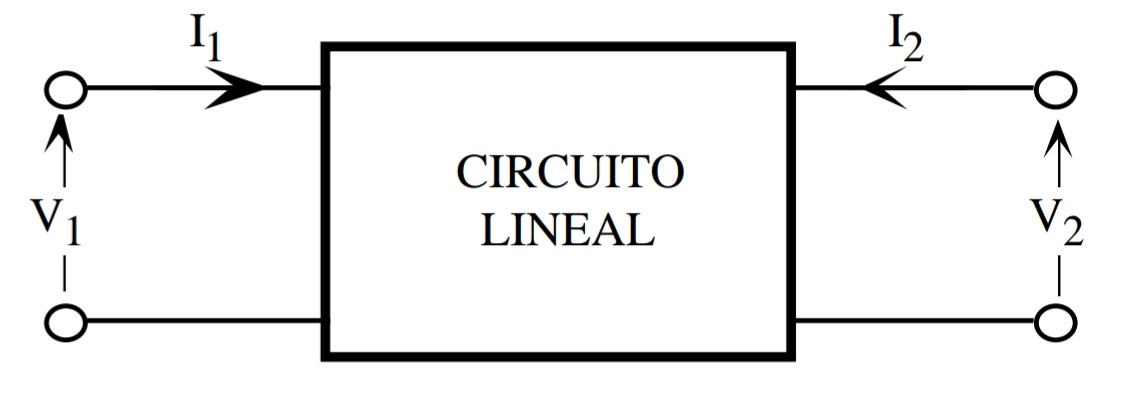
\includegraphics[height=4cm\textwidth]{circuito-lineal.jpg}
        \caption{Red bi-puerta}
        \label{fig:cir-lin}
    \end{figure}

    \subsection{Teoría de redes bipuerta}

    El comportamiento de un circuito lineal bi-puerta, tal como se muestra en la figura \ref{fig:cir-lin}, puede ser especificado a través de dos corrientes $(I_1, I_2)$ y dos tensiones $(V_1, V_2)$. En función de las dos posibles variables seleccionadas como independientes, ese circuito lineal puede ser caracterizado mediante cuatro tipo de parámetros ($\{Z\}, \{Y\}, \{H\}, \{G\}$), que en notación matricial, se expresan de la siguiente manera

    \begin{center} \par
        \begin{array}{c c}
            \begin{bmatrix}
                V_1 \\ 
                V_2 \\
            \end{bmatrix} = 
            \begin{bmatrix}
                z_i & z_r \\
                z_f & z_o
            \end{bmatrix}
            \begin{bmatrix}
                I_1 \\
                I_2
            \end{bmatrix} & 
            \begin{bmatrix}
                I_1 \\
                I_2 \\
            \end{bmatrix} = 
            \begin{bmatrix}
                y_i & y_r \\
                y_f & y_o
            \end{bmatrix}
            \begin{bmatrix}
                V_1 \\ 
                V_2 \\
            \end{bmatrix} \\
    
            \begin{bmatrix}
                V_1 \\ 
                I_2 \\
            \end{bmatrix} = 
            \begin{bmatrix}
                h_i & h_r \\
                h_f & h_o
            \end{bmatrix}
            \begin{bmatrix}
                I_1 \\
                V_2
            \end{bmatrix} & 
            \begin{bmatrix}
                I_1 \\
                V_2 \\
            \end{bmatrix} = 
            \begin{bmatrix}
                g_i & g_r \\
                g_f & g_o
            \end{bmatrix}
            \begin{bmatrix}
                V_1 \\ 
                I_2 \\
            \end{bmatrix} \\
        \end{array}
    \end{center} \par
    
    Los parámetros $\{H\}$ o h o híbridos son los que mejor caracterizan el comportamiento lineal de pequeña señal de un transistor bipolar. Estos parámetros relacionan la $V_1$ e $I_2$ con la $I_1$ y $V_2$ mediante la siguiente ecuación
    
    \begin{equation*}
        \begin{split}
            V_1 & = h_iI_1 + h_rV_2 \\
            I_2 & = h_fI_1 + h_oV_2 \\
        \end{split}
    \end{equation*}

    donde

    [W] $h_i = \frac{V_1}{I_1}\|_{V_2 = 0}$ = resistencia de entrada con salida en cortocircuito.

    [NO] $h_r = \frac{V_1}{V_2}\|_{I_1 = 0}$ = ganancia inversa de tensi n con entrada en circuito abierto

    [NO] $h_f = \frac{I_2}{I_1}\|_{V_2 = 0}$ = ganancia de corriente con salida en cortocircuito

    [$W^{-1}$] $h_o = \frac{V_1}{V_2}\|_{I_1 = 0}$ = conduc tan cia de salida con entrada en circuito abierto

    El modelo circuital en parámetros h de un circuito lineal se indica en la figura \ref{fig:h}.


    \begin{figure}[h!]
        \centering
        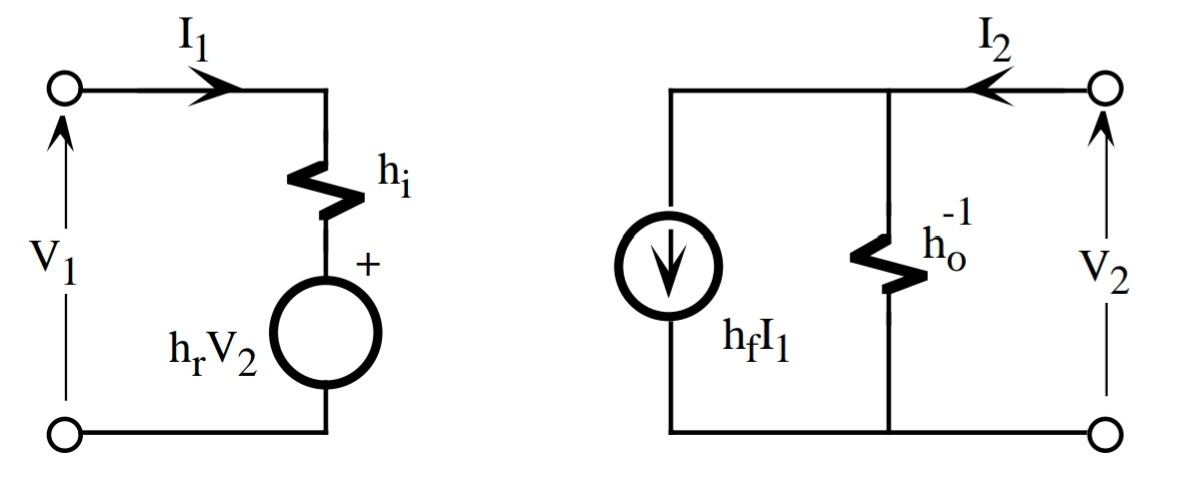
\includegraphics[height=4cm\textwidth]{parametrosh.jpg}
        \caption{Modelo equivalente en parámetros h.}
        \label{fig:h}
    \end{figure}

    \subsection{Análisis de un circuito empleando parámetros $\{H\}$}

    Un circuito lineal, por ejemplo un transistor actuando como amplificador, puede ser analizado estudiando su comportamiento cuando se excita con una fuente de señal externa VS con una impedancia interna RS y se añade una carga ZL, tal como se indica en la figura \ref{fig:amp-bas}. El circuito lineal puede ser sustituido por su modelo equivalente en parámetros {H} (figura \ref{fig:h}) resultando el circuito de la figura \ref{fig:amp-bas-h}. Existen cuatro parámetros importantes que van a caracterizar completamente el circuito completo: ganancia en corriente, impedancia de entrada, ganancia en tensión e impedancia de salida.

    \begin{figure}[h!]
        \centering
        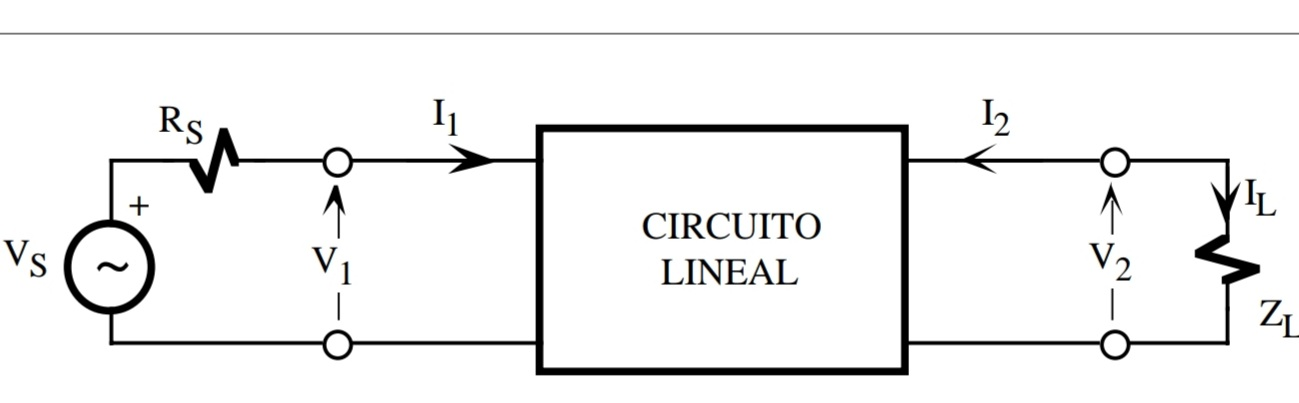
\includegraphics[height=4cm\textwidth]{amp-bas.jpg}
        \caption{Estructura de un amplificador básico}
        \label{fig:amp-bas}
    \end{figure}

    \begin{figure}[h!]
        \centering
        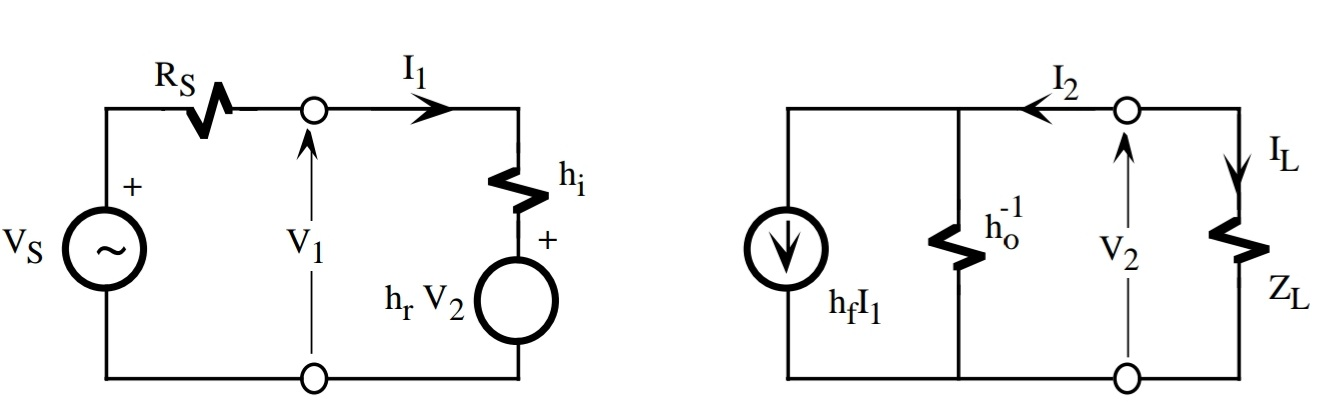
\includegraphics[height=4cm\textwidth]{amp-bas-h.jpg}
        \caption{Anterior circuito utilizando el modelo en parámetros h}
        \label{fig:amp-bas-h}
    \end{figure}

    \underline{\bf Ganancia de corriente.} Se define la ganancia de corriente de un circuito, AI, como la relación entre la intensidad de salida e intensidad de entrada, es decir,

    $$A_I = {I_L \over I_1} = -{I_2 \over I_1}$$

    Este cociente se obtiene resolviendo las siguientes ecuaciones extraidas del circuito de la figura \ref{fig:amp-bas-h},

    \begin{equation*} %pendiente
        \left\{ \begin{split}
            I_2 & = h_fI_1 + h_oV_2 \\
            V_2 & = -I_2Z_L 
        \end{split} \right.
    \end{equation*}

    Despejando, se obtiene que

    $$A_I = -{I_2 \over I_1} = -\frac{h_f}{1 + h_oZ_L}$$

    \underline{\bf Impedancia de entrada.} Se define la impedancia de entrada del circuito, $Z_i$, como la relación entre la tensión y corriente de entrada. Resolviendo el circuito de entrada se demuestra que

    $$Z_i = {V_1 \over I_1} = h_i + h_rA_IZ_L = h_i + \frac{h_fh_r}{{1 \over Z_L} + h_o}$$

    Nótese que la impedancia de entrada depende de la carga $Z_L$.

    \underline{\bf Ganancia de tensión.}  Se define la ganancia en tensión, AV, como la relación entre la tensión de salida y la tensión de entrada. Como se demuestra a continuación, la AV se puede expresar en función de la AI y la Zi, de forma que

    \begin{equation}
        A_v = {V_2 \over V_1} = {V_2 \over I_2}{I_2 \over I_1}{I_1 \over V_1} = -{V_2 \over I_L}{I_2 \over I_1}{I_1 \over V_1} = Z_LA_I{1 \over Z_i} = A_I{Z_L \over Z_i}
        \label{ganancia}
    \end{equation}

    \underline{\bf Impedancia de salida.} Se define la impedancia de salida, $Z_o$, vista a través del nudo de salida del circuito lineal como la relación entre la tensión de salida y la corriente de salida, supuesto anulado el generador de entrada y en ausencia de carga $(Z_L = \infty)$. Se demuestra que

    $$Z_o = {V_2 \over I_2}|_{V_S = 0, R_L = \infty} = \frac{1}{h_o - {h_fh_r \over R_S + h_i}}$$

    Estos cuatro parámetros permiten definir dos modelos simplificados muy utilizados en al análisis de amplificadores: modelo equivalente en tensión y modelo equivalente en intensidad. El modelo equivalente en tensión (figura \ref{fig:mod-ten}) utiliza el equivalente Thèvenin en la salida y el de intensidad (figura \ref{fig:mod-int}) el Norton. Ambos modelos son equivalentes y están relacionados por la ecuación \ref{ganancia}.

    \begin{figure}[h!]
        \centering
        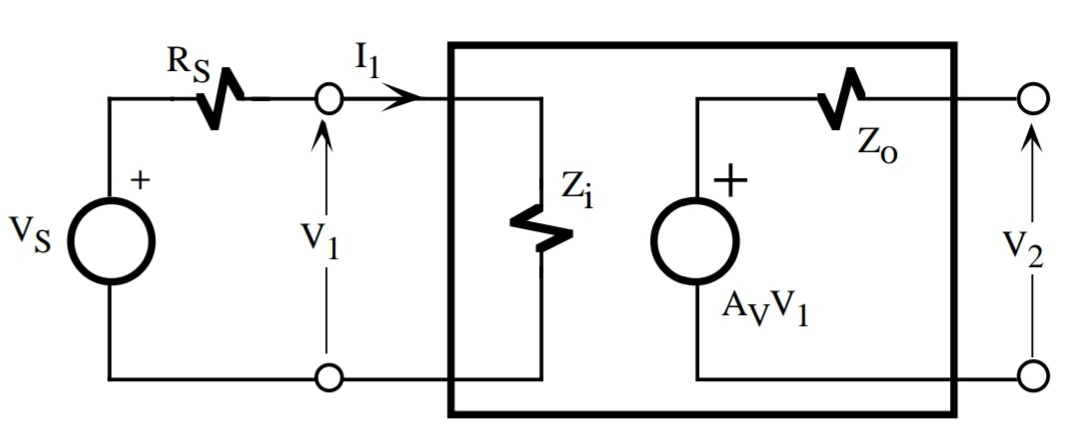
\includegraphics[height=4cm\textwidth]{mod-ten.jpg}
        \caption{Modelo equivalente en tensión}
        \label{fig:mod-ten}
    \end{figure}

    \begin{figure}[h!]
        \centering
        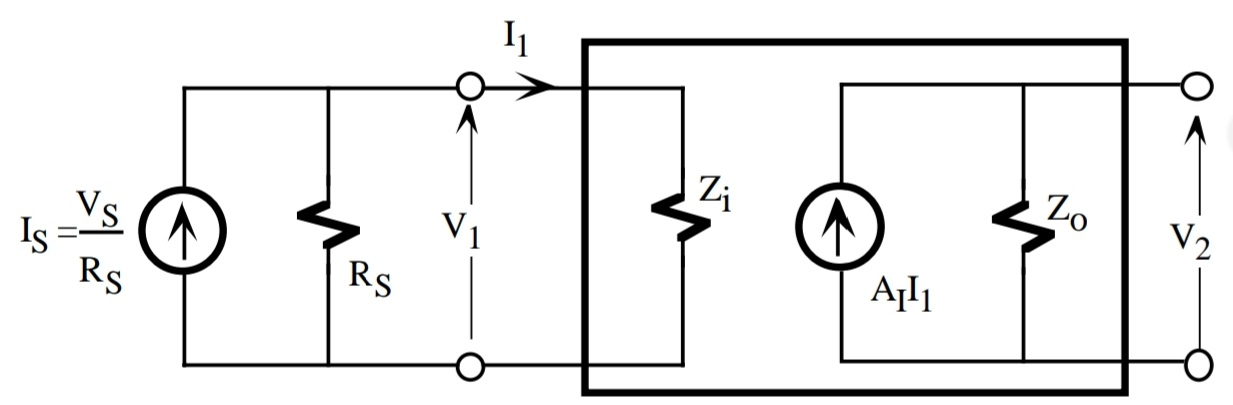
\includegraphics[height=4cm\textwidth]{mod-int.jpg}
        \caption{Modelo equivalente en intensidad}
        \label{fig:mod-int}
    \end{figure}

    La resistencia $R_S$ de la fuente de entrada influye en las expresiones de las ganancias de tensión o intensidad cuando se refieren a la fuente de excitación de entrada. En la figura \ref{fig:mod-ten}, la ganancia de tensión referida a la fuente $V_S$, $A_{VS}$, se obtiene analizando el divisor de tensión de la entrada formado por $R_S$ y $Z_i$, resultando

    $$A_{VS} = {V_2 \over V_S} = {V_2 \over V_1}{V_1 \over V_S} = A_V \frac{Z_i}{Z_i + R_S}$$

    De la misma manera, la ganancia de intensidad referida a la fuente IS (figura \ref{fig:mod-int}), $A_IS$, se obtiene analizando el divisor de corriente de entrada formado por $R_S$ y $Z_i$, resultando

    $$A_{IS} = {I_L \over I_S} = {I_L \over I_1}{I_1 \over I_S} = A_I \frac{R_S}{Z_i + R_S}$$

    Despejando en de la últimas dos ecuaciones $A_V$ y $A_I$, y sustituyendo en \ref{ganancia}, se obtiene la relación entre $A_{VS}$ y $A_{IS}$, dando como resultado

    $$A_{VS} = A_{IS}{Z_L \over R_S}$$

    \newpage

    \section{Metodología}

    \subsection{Trabajo Previo al Laboratorio}

    La estructura básica amplificadora corresponde al circuito de la Figura \ref{fig:circuito} sin RL y CE. Para éste circuito se realizó lo siguiente:

    \begin{figure}[h!]
        \centering
        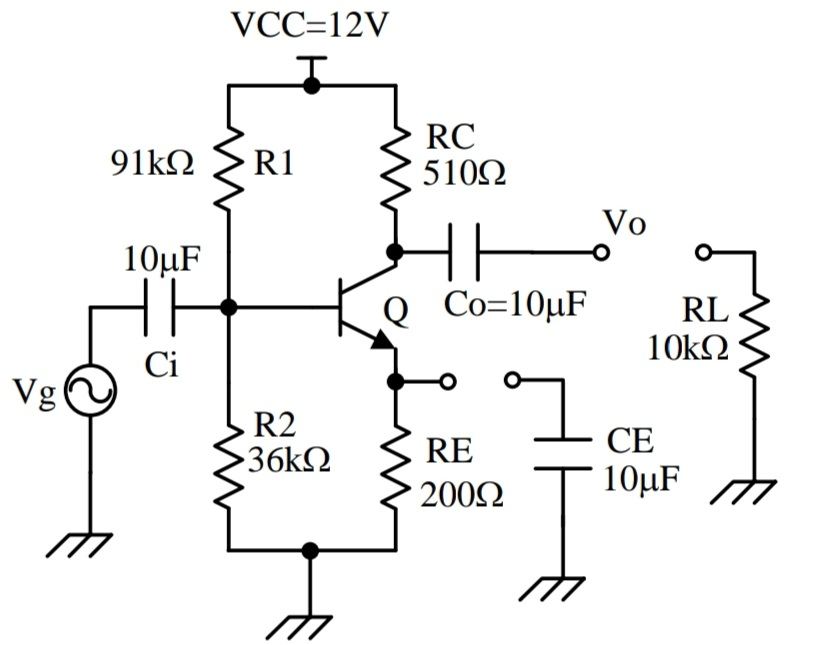
\includegraphics[height=5cm\textwidth]{amplificadorbjt.jpg}
        \caption{Amplificador Básico BJT}
        \label{fig:circuito}
    \end{figure}

    \begin{enumerate}
        \item Se determinó el punto estático de operación. \label{p1}
        \item Se calculó, utilizando los parámetros híbridos del transistor, la ganancia de tensión $A_V$, impedancia de entrada $Z_{in}$ y la impedancia de salida $Z_o$. \label{p2} %pendiente p2
        \item Se colovó la resistencia de carga RL y se repitió el punto 1 \ref{p2}.
        \item Sin RL, se colocó un condensador paralelo a la resistencia RE y se repitió el punto \ref{p2}.
        \item Con RL y CE se repitió el punto \ref{p2}.
    \end{enumerate}

    \subsection{Trabajo de Laboratorio}

    \begin{enumerate}
        \item Para el circuito de la Figura \ref{fig:circuito}, sin el generador de entrada (Vg), los condensadores (Ci, Co y CE) y la carga RL, se midió la tensión en el Colector ($V_C$), tensión en la Base ($V_B$) y la tensión en el Emisor ($V_E$) para determinar el punto estático de operación en el informe.
        \item \underline{Amplificador básico de la Figura \ref{fig:circuito} sin RL y CE.} \label{lab1}
        \begin{enumerate}
            \item Se colocó en el generador una señal senoidal de frecuencia 1kHz, promedio nulo y amplitud 2Vp-p. Se conectó los condensadores Ci, Co y el generador de entrada (Vg).\label{p21}
            \item Con el osciloscopio en DC, se capturó la señal en el Colector del transistor. Se midió la amplitud pico-pico, la tensión pico máxima y el nivel DC de la onda. \label{p22}
            \item Con el osciloscopio en AC en ambos canales y en doble canal. Se capturó la onda de la entrada (Vg) y la salida (Vo). Se midió la frecuencia y amplitud pico-pico de las ondas para luego determinar la ganancia de tensión Av en el informe.
            \item Se midió experimentalmente los valores de tensiones para luego determinar en el informe las impedancias de entrada y de salida del amplificador.
            \item Se subió la amplitud de la señal de entrada hasta el punto donde comienza a distorsionarse la señal de salida. Se midió la amplitud pico-pico de la señal de salida y de entrada. Dibuje ambas formas de onda.
            \item Se subió hasta el máximo la amplitud de la señal de entrada y se midió ésta amplitud pico-pico. Se dibujó las ondas. \label{p26}
        \end{enumerate}
        \item \underline{Amplificador básico de la Figura \ref{fig:circuito} con RL y sin CE.} \label{lab2}
        \begin{enumerate}
            \item Con las mismas condiciones colocadas en el punto \ref{p21}, se repitió los puntos \ref{p22} hasta \ref{p26}.
        \end{enumerate}
        \item \underline{Amplificador básico de la Figura \ref{fig:circuito} sin RL y con CE.} \label{lab3}
        \begin{enumerate}
            \item Con las mismas condiciones colocadas en el punto \ref{p21}, se repitió los puntos \ref{p22} hasta \ref{p26}.
        \end{enumerate}
        \item \underline{Amplificador básico de la Figura \ref{fig:circuito} con RL y con CE.} \label{lab4}
        \begin{enumerate}
            \item Con las mismas condiciones colocadas en el punto \ref{p21}, se repitió los puntos \ref{p22} hasta \ref{p26}.
        \end{enumerate}
    \end{enumerate}

    \newpage

    \section{Cálculos prévios}

    Se trabajará con el transistor npn PN2222A, el cual posee las siguientes especificaciones:

    \begin{table}[h!]
        \centering
        \caption{Características del transistor PN2222A} %nombre de la tabla
        \label{tab:especificaciones} %indice de la tabla
        \begin{tabular}{c}
            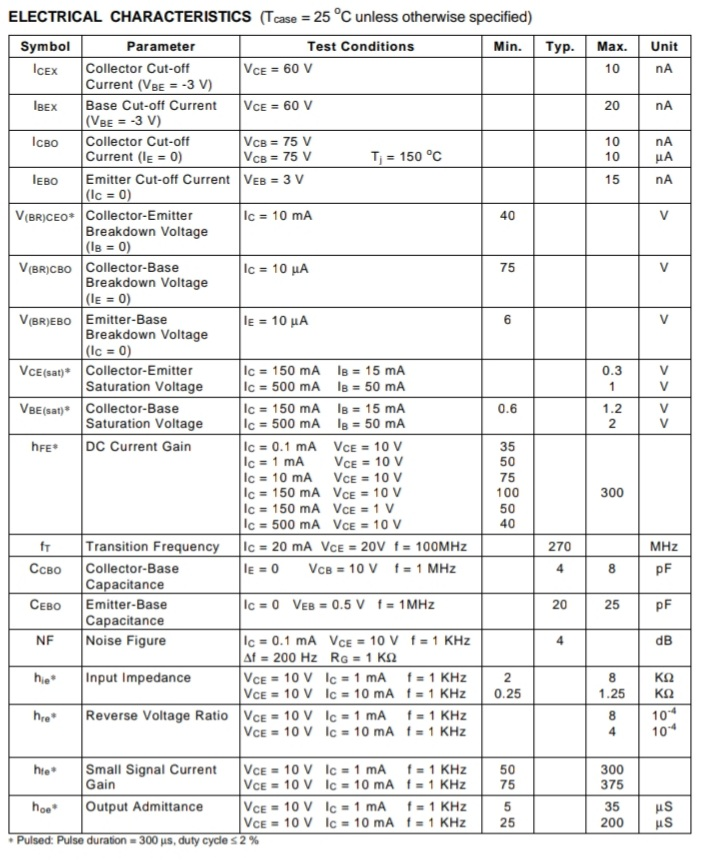
\includegraphics[height=20cm\textwidth]{pn2222a.jpg} \\
        \end{tabular}
    \end{table}
    
    de las cuales se deduce que:

    $\beta = h_{FE} = 150 \; @ \; I_C = 10mA; \; V_{CE} = 10V$

    $V_{BEsat} = 0.7V \; @ \; I_C = 150mA; \; I_B = 10mA$

    $h_{ie} = 5K\Omega \; @ \; I_C = 1mA; \; V_{CE} = 10V; \; f = 1KHz$

    $h_{fe} = 175 \; @ \; I_C = 1mA; \; V_{CE} = 10V; \; f = 1KHz$

    Se determina el punto estático de operacion basandose en el circuito de la Figura \ref{fig:1}

    \begin{figure}[h!]
        \centering
        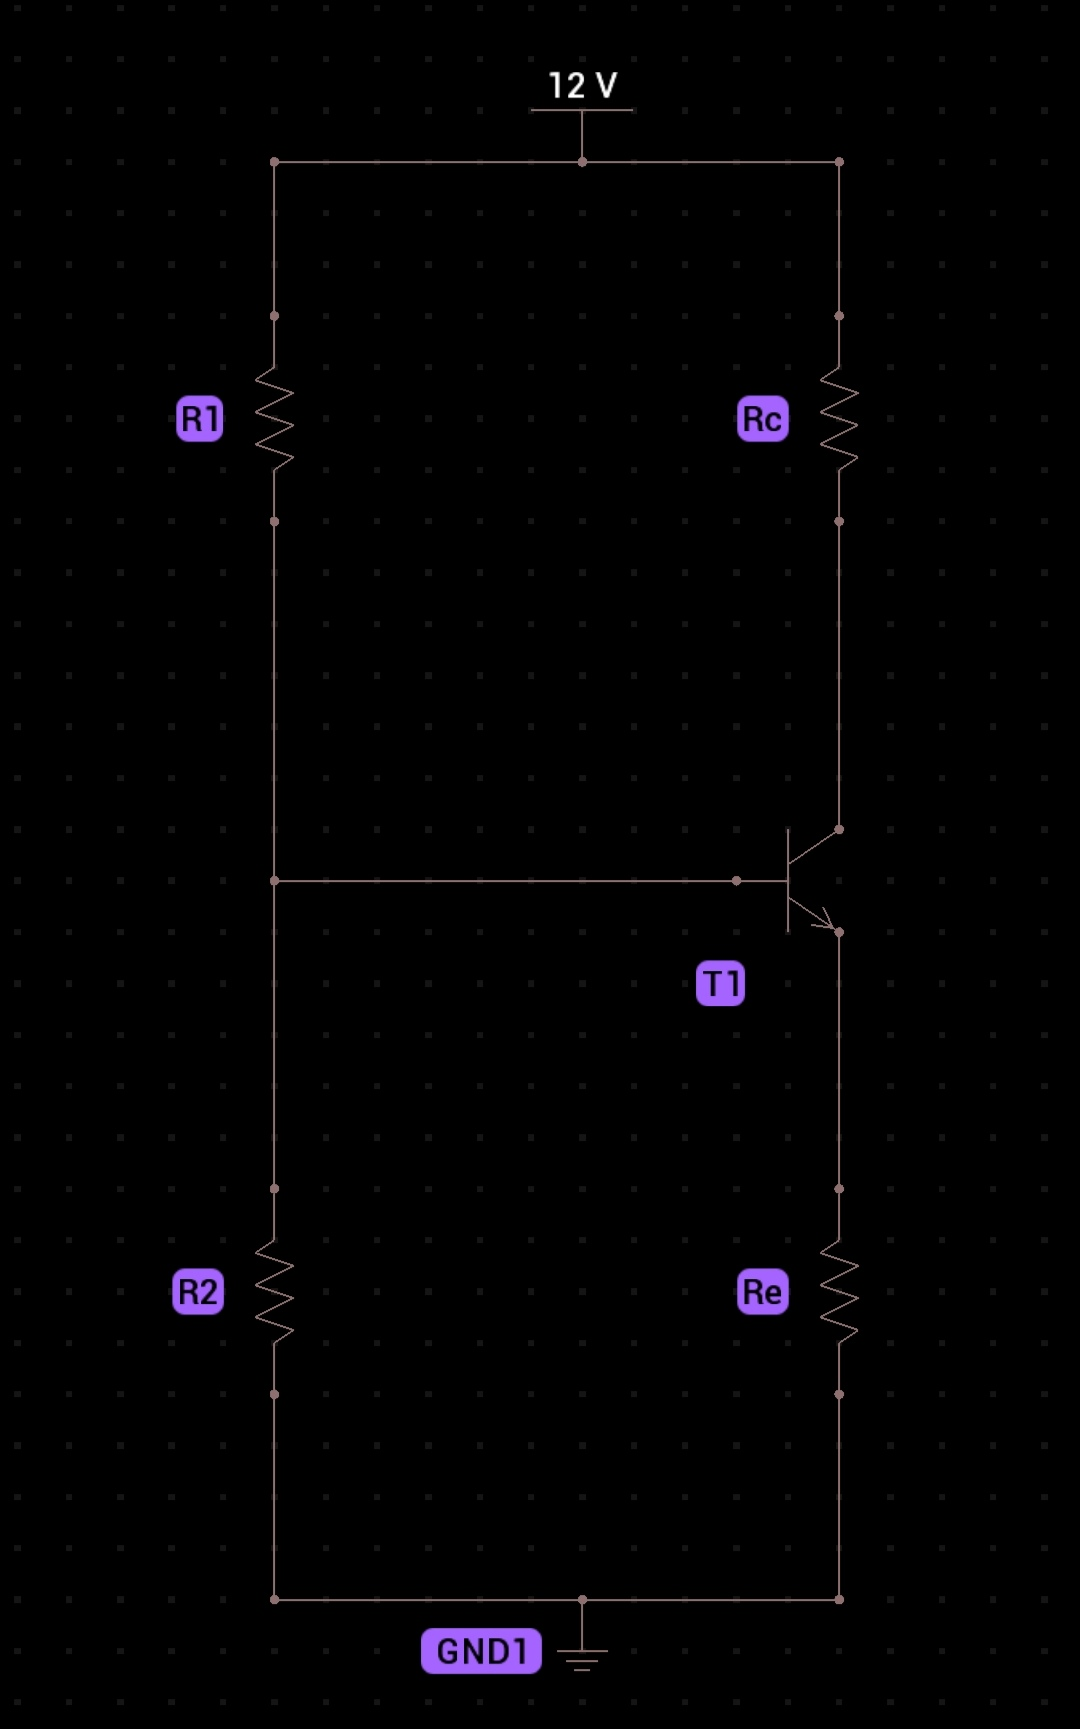
\includegraphics[height=4cm\textwidth]{qestatico.jpg}
        \caption{Circuito de operación estática}
        \label{fig:1}
    \end{figure}

    Calculando equivalente de thevelin entre la base del transistor y la referencia
    
    \begin{split}
        R_{Th} & = R_1 || R_2 = \frac{R_1R_2}{R_1 + R_2} \\
        R_{Th} & = \frac{(91K\Omega)(36K\Omega)}{91K\Omega + 36K\Omega} = 25.8K\Omega
    \end{split}
    
    por divisor de voltaje

    \begin{split}
        V_{Th} & = \frac{R_2}{R_1 + R_2} V_{CC} \\
        V_{Th} & = \frac{36K\Omega}{91K\Omega + 36K\Omega} (12V) = 3.4V
    \end{split}

    \begin{figure}[h!]
        \centering
        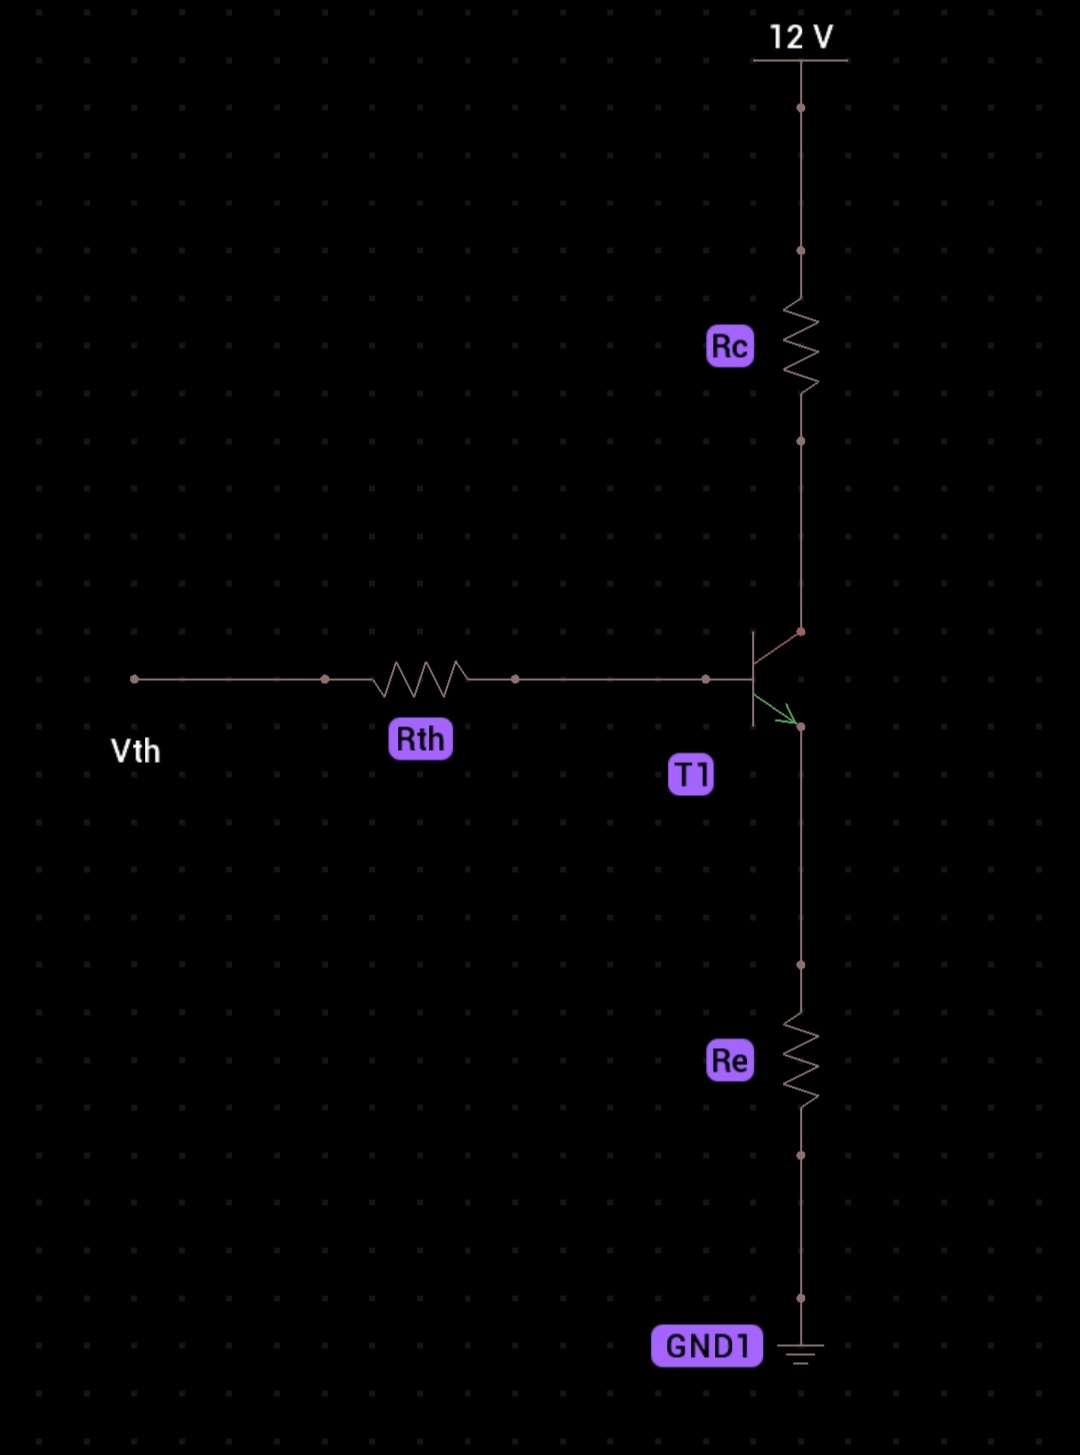
\includegraphics[height=4cm\textwidth]{thqestatico.jpg} \par
        \caption{Circuito de operación estática simplificado Thevelin}
        \label{fig:2}
    \end{figure}

    aplicando ley de tensiones de Kirchoff

    $$R_{Th}I_B + V_{BE} + R_EI_E = V_{Th}$$

    si $I_E = (\beta + 1)I_B$, entonces

    $$R_{Th}I_B + V_{BE} + R_E(\beta + 1)I_B = V_{Th}$$

    $$I_B = {V_{Th} - V_{BE} \over R_{Th} + R_E(\beta + 1)}$$

    Sustituyendo valores

    $$I_B = {3.4V - 0.7V \over 25.8k\Omega + 200\Omega(150 + 1)} = 0.048mA$$

    sabiendo que $I_C = \beta I_B$

    $$I_C = 150(0.048mA) = 7.23mA$$

    aplicando ley de tensiones de Kirchoff a la otra malla

    $$R_{C}I_C + V_{CE} + R_EI_E = V_{CC}$$

    $$V_{CE} = V_{CC} - R_{C}I_C - R_E(\beta + 1)I_B$$

    sustituyendo

    $$V_{CE} = 12V - 510\Omega (7.23mA) - 200\Omega (150 + 1) 0.048mA = 6.86V$$

    Punto de operacion

    \begin{equation} \label{eqQ}
        \begin{split}
            Q & = (V_{CE}, I_C) \\
            Q & = (6.86V, 7.23mA) \\
        \end{split}
    \end{equation}

    Por lo tanto se puede decir que está trabajando en la zona activa y en consecuencia puede amplificar una señal.

    Utilizando el modelo de parametros híbridos de la Figura \ref{fig:h1} sin tomar en cuenta RL ni CE

    \begin{figure}[h!]
        \centering
        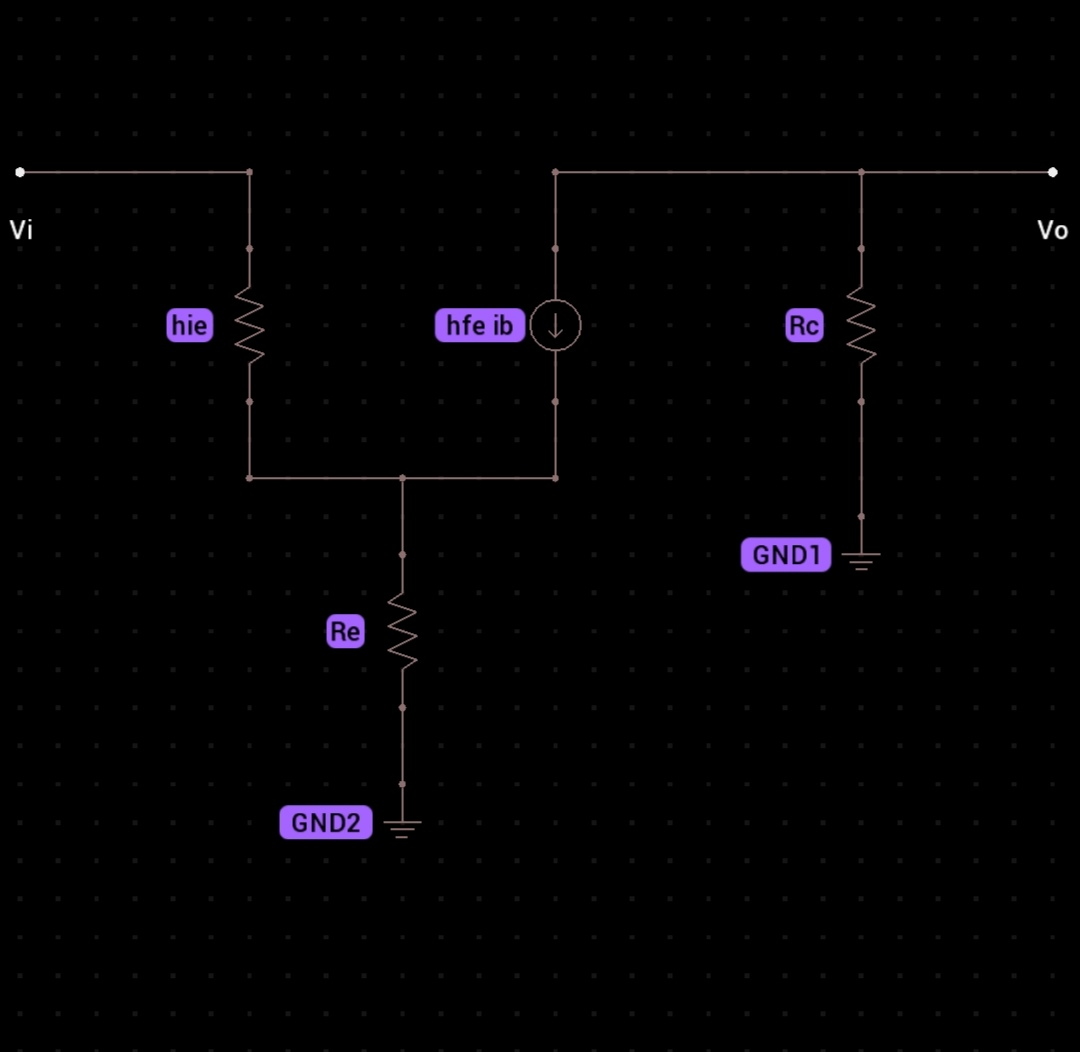
\includegraphics[height=4cm\textwidth]{h1.jpg} \par
        \caption{Modelo de parametros híbridos sin RL ni CE}
        \label{fig:h1}
    \end{figure}

    Se puede apreciar en la figura \ref{fig:h1} que $R_1$ y $R_2$ actúa como un corto a tierra debido al capacitor que se encuentra en la entrada, donde se asume una señal media.

    Sabiendo que

    \begin{equation}
        A_V = {V_o \over V_i}
        \label{eq1}
    \end{equation}

    Además si

    $$V_i = i_bh_{ie} + (h_{fe}+1)i_bR_E = i_b(h_{ie} + (h_{fe}+1)R_E)$$

    $$V_o = -h_{fe}i_bR_C$$

    Sustituyendo lo anterior en la ecuacion \eqref{eq1}

    \begin{equation}
        A_V = -\frac{h_{fe}R_C}{h_{ie} + (h_{fe}+1)R_E}
        \label{eq2}
    \end{equation}

    Reemplazando parámetros

    $$A_V = -\frac{-(175)(510\Omega)}{5K\Omega + (175+1)(200\Omega)} = -2.22 V/V$$

    Para calcular las impedancias no se toma en cuenta el condensador acoplado, entonces:

    \begin{equation}
        Z_i = R_{Th}||Z_1
        \label{eq3}
    \end{equation}

    si

    $R_{Th} = R_1||R_2 = 25.8K\Omega$

    \begin{equation*}
        \begin{split}
            Z_1 & = {V_i \over i_b} = \frac{i_b(h_{ie} + (h_{fe}+1)R_E)}{i_b} = h_{ie} + (h_{fe}+1)R_E \\
            Z_1 & = 5K\Omega + (175+1)(200\Omega) = 40.2K\Omega
        \end{split}
    \end{equation*}

    sustituyendo en ecuación \eqref{eq3}

    $$Z_i = 25.8K\Omega||40.2K\Omega = 15.7K\Omega$$

    Además

    $$Z_o = R_C = 510\Omega$$
    
    Utilizando el modelo de parametros híbridos de la Figura \ref{fig:h2} tomando en cuenta solamente RL

    \begin{figure}[h!]
        \centering
        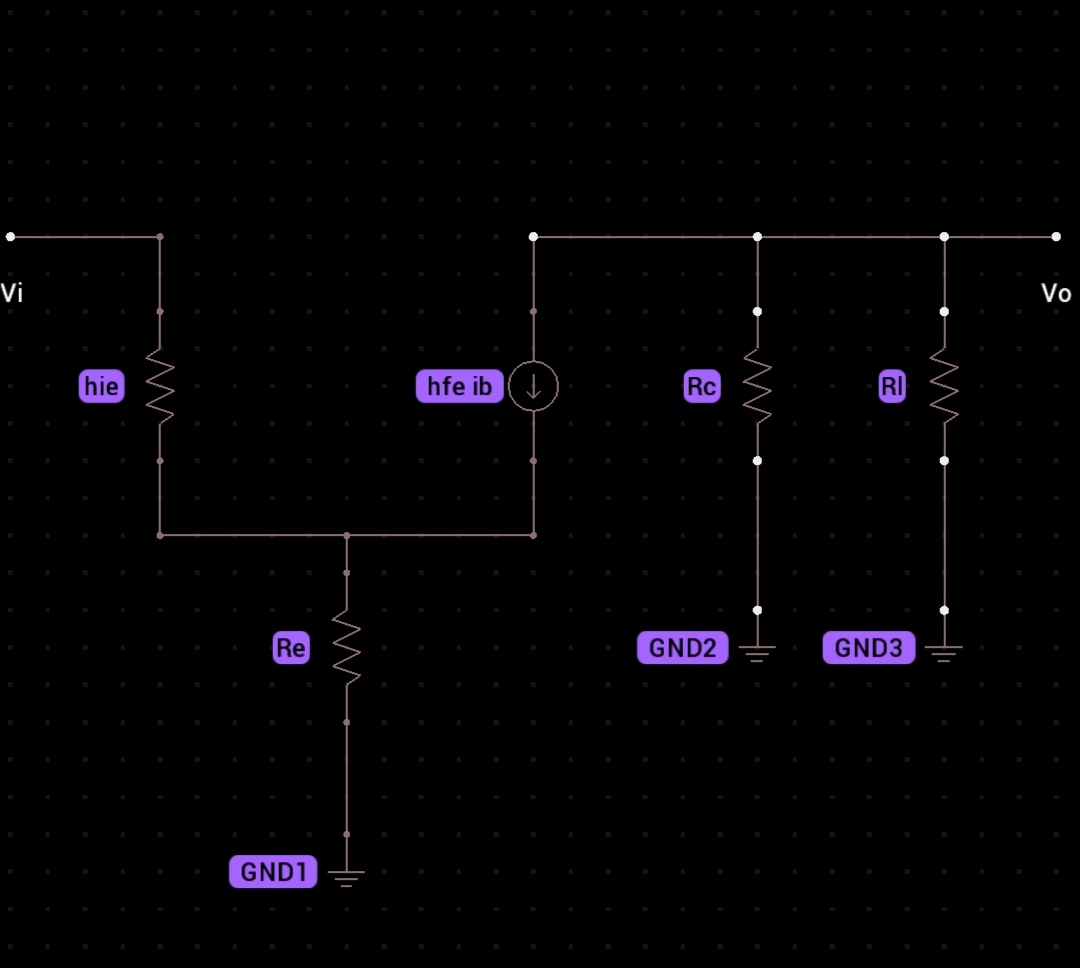
\includegraphics[height=4cm\textwidth]{h2.jpg} \par
        \caption{Modelo de parametros híbridos con RL}
        \label{fig:h2}
    \end{figure}

    Adaptando la ecuación \eqref{eq2} a

    \begin{equation}
        A_V = -\frac{h_{fe}R'_C}{h_{ie} + (h_{fe}+1)R_E}
        \label{eq4}
    \end{equation}

    donde
    
    \begin{equation*}
        \begin{split}
            R'_C & = R_C||R_L = \frac{R_CR_L}{R_C + R_L} \\
            R'_C & = \frac{(510\Omega)(10K\Omega)}{510\Omega + 10K\Omega} = 485\Omega
        \end{split}
    \end{equation*}   

    Reemplazando valor en la ecuación \eqref{eq4}

    $$A_V = -\frac{-(175)(485\Omega)}{5K\Omega + (175+1)(200\Omega)} = -2.11 V/V$$

    Ya que la entrada no se ve afectada por RL, la impedancia de entrada $Z_i$ nom sufre modificación

    $$Z_i = 15.7K\Omega$$

    Para la impedancia de salida

    $$Z_o = R'_C = 485\Omega$$

    Utilizando el modelo de parametros híbridos de la Figura \ref{fig:h2} tomando en cuenta solamente CE

    \begin{figure}[h!]
        \centering
        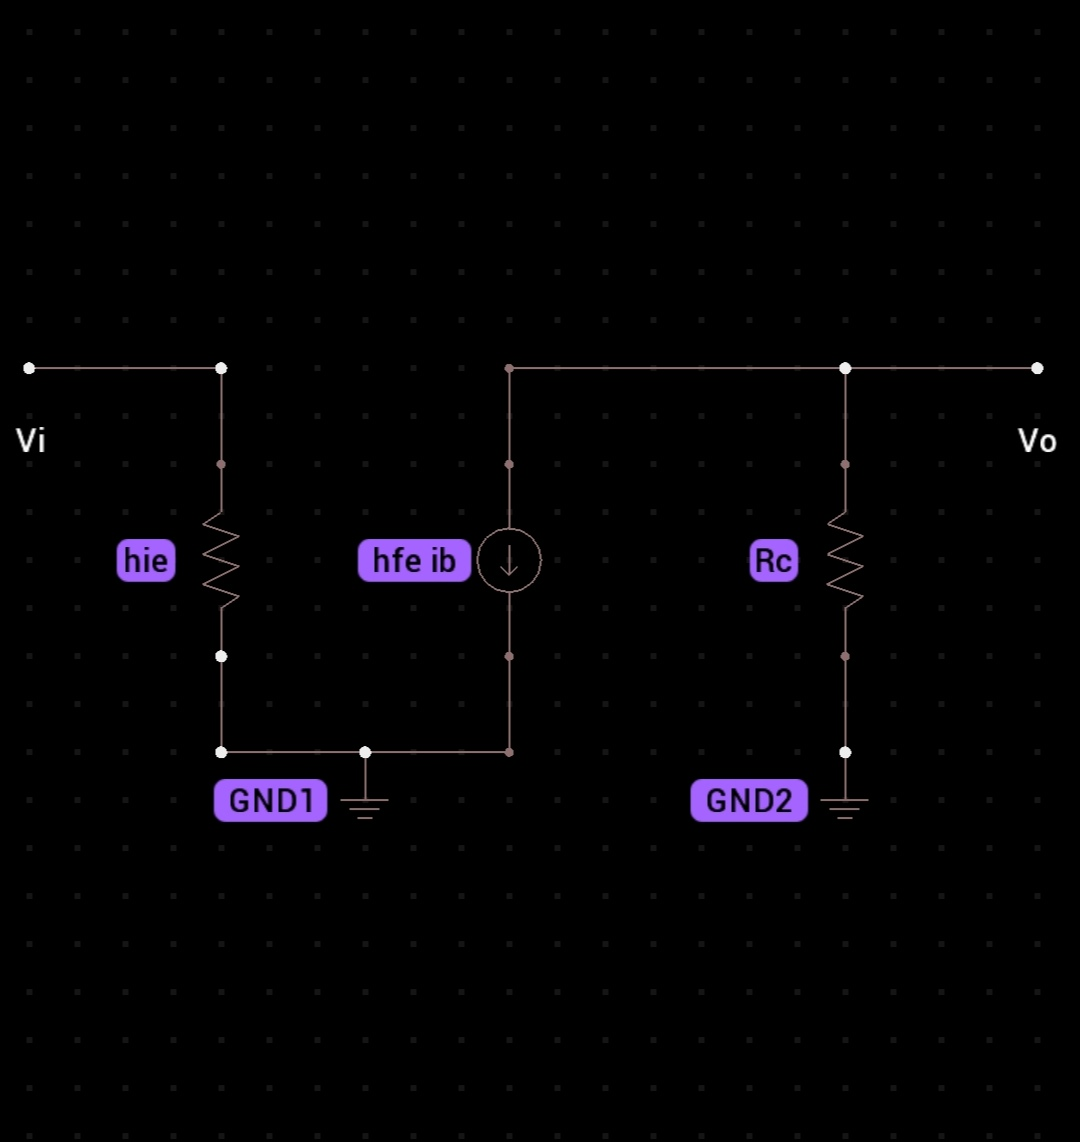
\includegraphics[height=4cm\textwidth]{h3.jpg} \par
        \caption{Modelo de parametros híbridos con CE}
        \label{fig:h3}
    \end{figure}

    Sabiendo que

    $V_i = h_{ie}i_b$

    $V_o = -h_{fe}i_bR_C$

    Reemplazando en ecuación \eqref{eq1} se demuestra que

    \begin{equation}
        A_V = -{h_{fe}R_C \over h_{ie}}
        \label{eq5}
    \end{equation}

    sustituyendo parametros

    $$A_V = -{(175)(510\Omega) \over 5K\Omega} = -17.85 V/V$$

    Para el cálculo de la impedancia de entrada se hace uso de la ecuación \eqref{eq3}, donde

    \begin{equation*}
        \begin{split}
            Z_1 & = {V_i \over i_b} = \frac{i_bh_{ie}}{i_b} = h_{ie} \\
            Z_1 & = 5K\Omega
        \end{split}
    \end{equation*}  

    sustituyendo en \eqref{eq3}

    $$Z_i = R_{Th}||Z_1 = 25.8K\Omega||5K\Omega = 4.2K\Omega$$

    Además

    $$Z_o = R_C = 510\Omega$$

    \begin{figure}[h!]
        \centering
        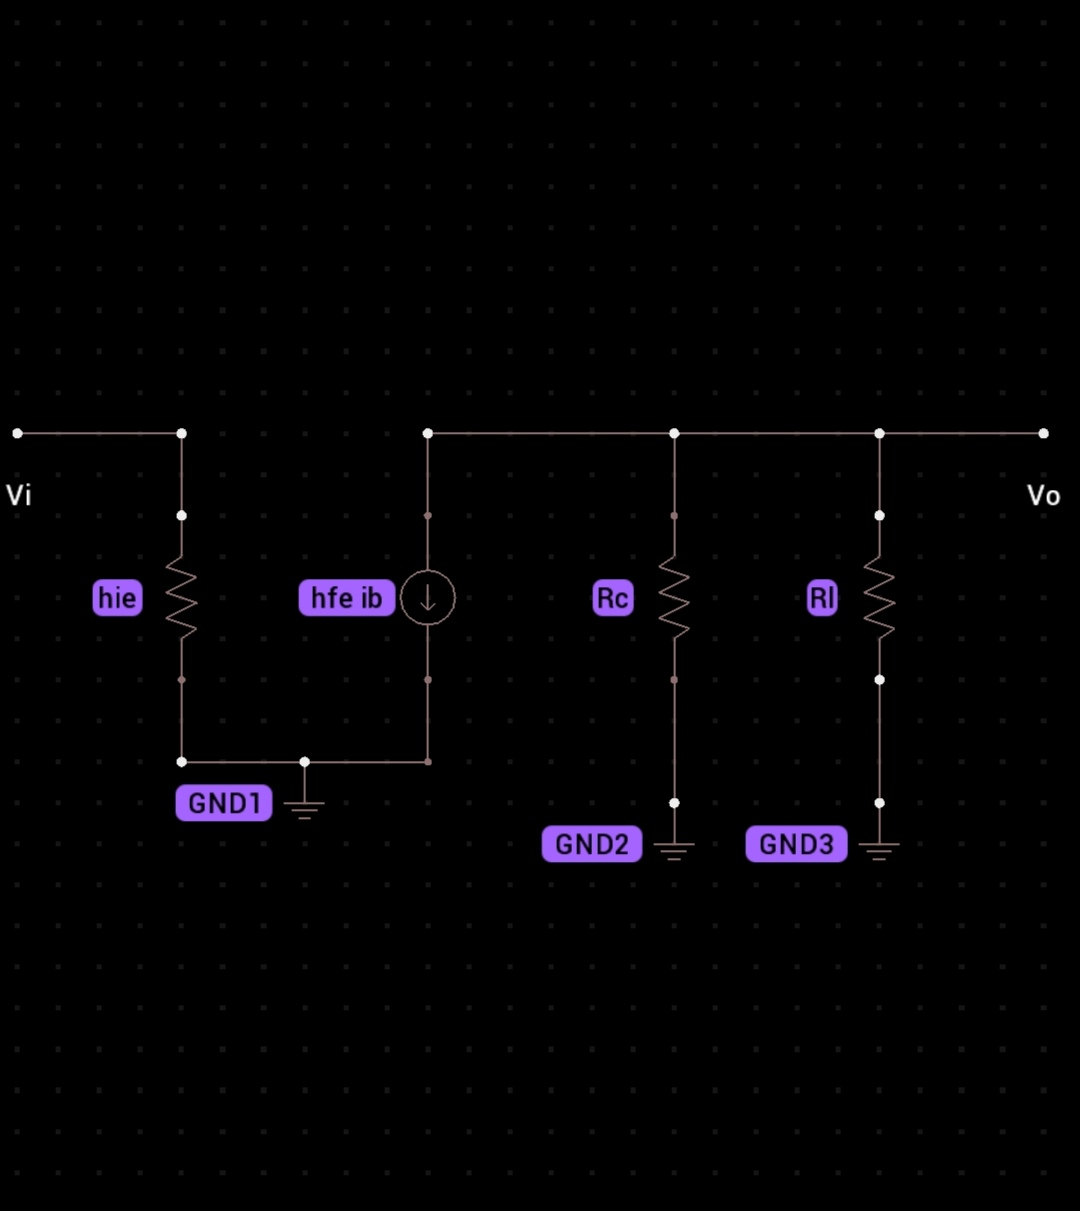
\includegraphics[height=4cm\textwidth]{h4.jpg} \par
        \caption{Modelo de parametros híbridos con RL y CE}
        \label{fig:h4}
    \end{figure}

    Adaptando \ref{eq5}

    \begin{equation}
        A_V = -{h_{fe}R'_C \over h_{ie}}
        \label{eq6}
    \end{equation}

    donde $R'_C = 485\Omega$, ya calculado antes

    entonces en \ref{eq6}

    $$A_V = -{(175)(485\Omega) \over 5K\Omega} = -16.98V/V$$

    La impedancia de entrada $Z_i$ no cambia con respecto a la calculada en el caso anterior

    $$Z_i = 4.2K\Omega$$

    Además

    $$Z_o = R'_C = 485\Omega$$

    \begin{table}[h!]
        \centering
        \caption{Resultados teóricos}
        \label{tab:rteo}
        \begin{tabular}{|c|c|c|c|} \hline
            Prueba de lab.    &    $A_V$     &    $Z_i$      &  $Z_o$   \\ \hline
            \ref{lab1}     &  -2.22 V/V   &   15.7K\Omega &  510\Omega \\
            \ref{lab2}   &  -2.11 V/V   &   15.7K\Omega &  485\Omega \\
            \ref{lab3}   &  -17.85 V/V  &   4.2K\Omega &  510\Omega \\
            \ref{lab2}     &  -16.98V/V  &   4.2K\Omega &  485\Omega  \\ \hline
        \end{tabular}
    \end{table}

    \newpage
    \newpage

    \section{Materiales e Instrumentos}

    \begin{table}[h!]
        \centering
        \caption{Equipos o instrumentos}
        \label{tab:instrumentos}
        \begin{tabular}{|c|c|c|} \hline
            Equipo                    &  Marca&    Modelo   \\ \hline
            Osciloscopio              &  UNI-T & UTD2102CEX+ \\ 
            Fuente de alimentacion DC  &  UNI-T & UTP3305-II  \\ \hline
        \end{tabular}
    \end{table}

    \begin{table}[h!]
        \centering
        \caption{Componentes y materiales}
        \label{tab:componentes}
        \begin{tabular}{|c|c|c|} \hline
            Referecia&Descripcion&    Especificaciones   \\ \hline
            R1 = 100k$\Omega$  &  Resistencia&         1/4 W         \\
            R2 = 36k$\Omega$   &  Resistencia&         1/4 W         \\
            RC = 510$\Omega$   &  Resistencia&         1/8 W         \\
            RE = 220$\Omega$   &  Resistencia&         1/4 W         \\
            $RP_Ri$ = 15k$\Omega$   &  Resistencia&         1/4 W         \\
            $RP_Ri$ = 5.1k$\Omega$   &  Resistencia&         1/4 W         \\
            $RP_Ro$ = 470$\Omega$   &  Resistencia&         1/4 W         \\
            Ci = Co = CE = 10$\mu F$ & Condensador Electrolítico & 25V \\
            Q = PN2222A    &Tansistor BJT NPN&   \\ \hline
        \end{tabular}
    \end{table}

    \newpage

    \section{Presentación de Resultados}

    \begin{table}[h!]
        \centering
        \caption{Tensiones en los terminales del transistor sin RL ni CE}
        \label{tab:Q}
        \begin{tabular}{|c|c|c|c|c|c|} \hline
            $V_B$ [V]  &  $V_C$ [V] &  $V_E$ [V]  &  $I_C$ [mA] & $V_{CE}$ [V] & operacion \\ \hline
            2.2 ± 0.2  &  9 ± 1     &  1.5 ± 0.1  &  5.88 ± 4.51  &  7.5 ± 1.1 & activo \\ \hline
        \end{tabular}
    \end{table}

    \begin{table}[h!]
        \centering
        \caption{Frecuencia de $V_g$}
        \label{tab:f}
        \begin{tabular}{|c|} \hline
            $f$ [Hz]   \\ \hline
            999.99400 ± 0.00005   \\ \hline
        \end{tabular}
    \end{table}

    {\bf Observación:} Para el cáculo del punto estático de operacion $Q : (V_{CE},I_c)$ se utilizaron las fórmulas \eqref{Qeq1}, \eqref{Qeq2}, \eqref{Qeq3} y \eqref{Qeq4} expresadas en los anexos.

    \begin{figure}[h!]
        \centering
        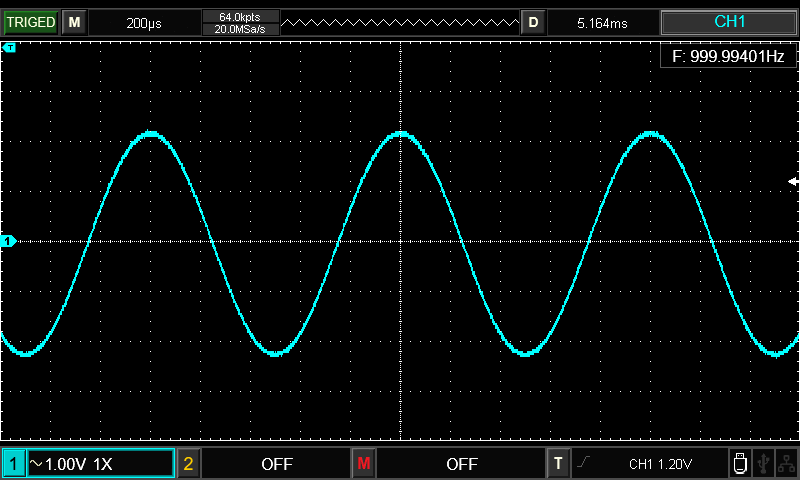
\includegraphics[height=5cm\textwidth]{Vg.png}
        \caption{Señal de entrada $V_g$ del circuito \ref{fig:circuito} predeterminada}
        \label{fig:vg}
    \end{figure}

    \begin{figure}[h!]
        \centering
        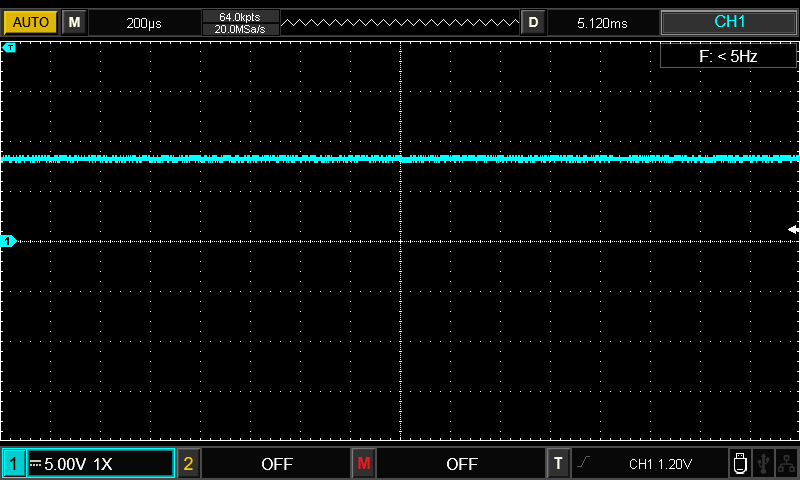
\includegraphics[height=5cm\textwidth]{VC.png}
        \caption{Tensión en colector $V_C$, componente DC de salida $V_o$ (fija para todas las configuraciones)}
        \label{fig:vc}
    \end{figure}

    \newpage

    \subsection{Prueba de laboratorio \ref{lab1} sin RL ni CE}

    \begin{figure}[h!]
        \centering
        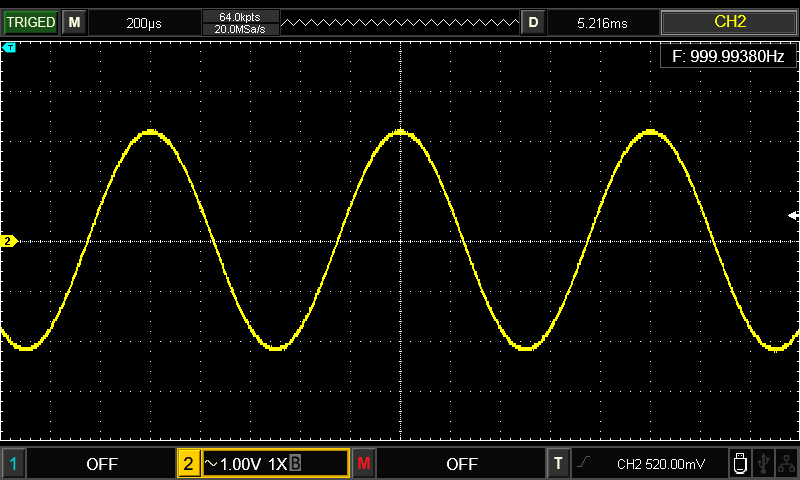
\includegraphics[height=5cm\textwidth]{VosRLsCE.png}
        \caption{Componente AC de señal de salida $V_o$ del circuito \ref{fig:circuito} original}
        \label{fig:voac}
    \end{figure}

    \begin{figure}[h!]
        \centering
        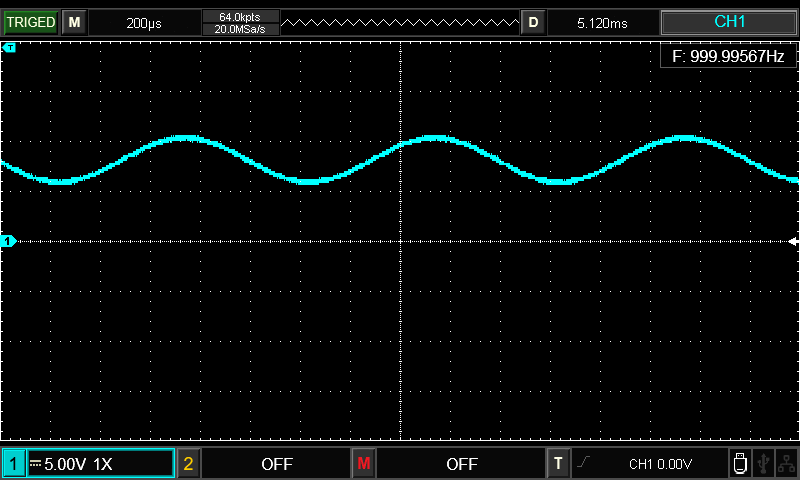
\includegraphics[height=5cm\textwidth]{VCsRLsCE.png}
        \caption{Superposición de señales DC y AC en la salida $V_o$}
        \label{fig:vo}
    \end{figure}

    \begin{figure}[h!]
        \centering
        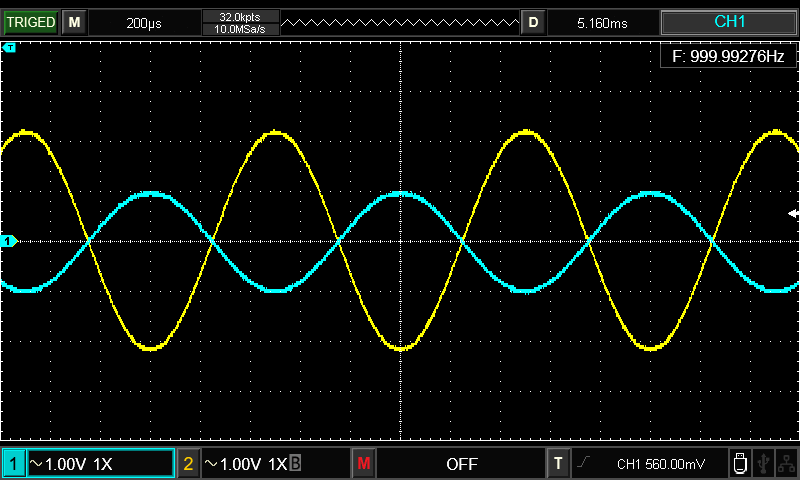
\includegraphics[height=5cm\textwidth]{ViosRLsCE.png}
        \caption{Señal de entrada $V_i$ (curva azul) y componete AC de señal de salida $V_o$ (curva amarilla)}
        \label{fig:vio1}
    \end{figure}

    \newpage

    Basandose en las señales de la figura \ref{fig:vio1} se recopilaron los siguientes datos

    \begin{table}[h!]
        \centering
        \caption{Tensiones pico-pico de entrada y salida sin RL ni CE}
        \label{tab:vio1}
        \begin{tabular}{|c|c|c|} \hline
            $V_i \; [V_{PP}]$  &  $V_o \; [V_{PP}]$   &  $V_{Pmax} [V]$\\ \hline
            2.0 ± 0.2            &       -4.4 ± 0.2     &  10.2 $\pm$ 1.2 \\ \hline
        \end{tabular}
    \end{table}

    {\bf Observación.} Para $V_{Pmax}$ se tomó el $V_o [V_P]$ en semiciclo positivo y se le sumó el escalón de la componente DC representada en la figura \ref{fig:vc}.

    Se calcularon las ganancias de tensión experimentales con la ecuacion \eqref{eqAv} referida en los anexos. Por otra parte, la ganancia teorica queda señalada en la tabla \ref{tab:rteo} en la sección de Cálculos prévios.

    \begin{table}[h!]
        \centering
        \caption{Ganancia relacionada al amplificador de la figura \ref{fig:circuito} sin RL ni CE}
        \label{tab:av1}
        \begin{tabular}{|c|c|c|} \hline
            $Av_{exp} \; [V/V]$  &  $Av_{teo} \; [V/V]$  & Desviación [\%] \\ \hline
            -2.20 ± 0.24         &       -2.22              & 1   \\ \hline
        \end{tabular}
    \end{table}

    \subsubsection{Implementando resistencias patrón ($R_P$) para cálculo de impeancias experimentales}

    Basandose en el modelo lineal de amplificador de la figura \ref{fig:rp} en la sección de anexos.

    \begin{table}[h!]
        \centering
        \caption{Resistencias patrones en circuito de la figura \ref{fig:circuito} sin RL ni CE}
        \label{tab:rp1}
        \begin{tabular}{|c|c|} \hline
            $R_{P_{Ri}}$          &  $R_{P_{Ro}}$  \\ \hline
            $15k\Omega \pm 10\%$  &  $470\Omega \pm 10\%$    \\ \hline
        \end{tabular}
    \end{table}

    \begin{figure}[h!]
        \centering
        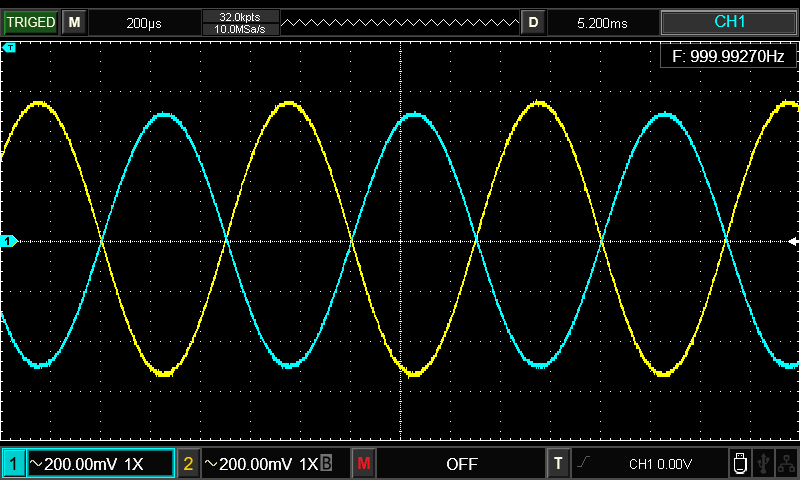
\includegraphics[height=5cm\textwidth]{RPsRLsCE.png}
        \caption{Señal $V_{R_{PRi}}$ (curva azul) y componete AC de señal de salida $V_{occ}$ (curva amarilla)}
        \label{fig:vrp1}
    \end{figure}

    \newpage

    De la figura \ref{fig:vrp1} se establecen los siguientes voltajes pico-pico

    \begin{table}[h!]
        \centering
        \caption{Tensiones pico-pico del terminal de las resistencias patrones asociadas a la figura \ref{fig:vrp1}}
        \label{tab:vrp1}
        \begin{tabular}{|c|c|} \hline
            $V_{R_i} [V_{PP}]$  &   $V_{occ} [V_{PP}]$  \\ \hline
            0.52 ± 0.04         &   0.56 ± 0.04    \\ \hline
        \end{tabular}
    \end{table}

    Sabiendo que $V_o = V_{osc}$ y utilizando las ecuaciones \eqref{eqri} y \eqref{eqro} de la sección de los anexos

    \begin{table}[h!]
        \centering
        \caption{Impedancia de entrada en circuito de la figura \ref{fig:circuito} sin RL ni CE}
        \label{tab:rpi1}
        \begin{tabular}{|c|c|c|} \hline
            $R_{i_{EXP}} [k\Omega]$  &   $R_{i_{TEO}} [k\Omega]$ & Desviación [\%]  \\ \hline
            16.25         &   15.7   & 4 \\ \hline
        \end{tabular}
    \end{table}

    \begin{table}[h!]
        \centering
        \caption{Impedancias de salida en circuito de la figura \ref{fig:circuito} sin RL ni CE}
        \label{tab:rpo1}
        \begin{tabular}{|c|c|c|} \hline
            $R_{o_{EXP}} [\Omega]$  &   $R_{o_{TEO}} [\Omega]$ & Desviación [\%]  \\ \hline
            1376         &   510   & 170 \\ \hline
        \end{tabular}
    \end{table}

    \begin{figure}
        \centering
        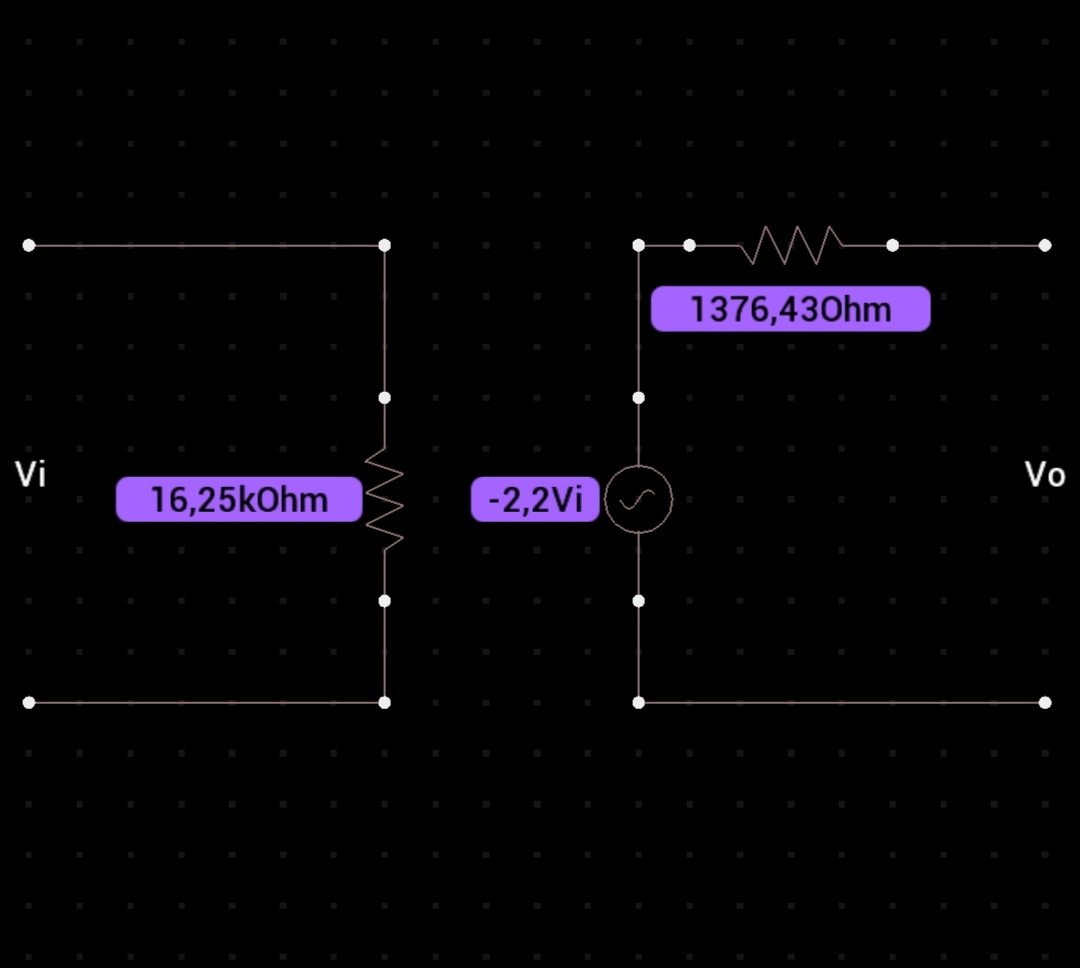
\includegraphics[height=5cm\textwidth]{ma1.jpg}
        \caption{Modelo lineal de amplificador de tensión para circuito de la figura \ref{fig:circuito} sin RL ni CE}
        \label{fig:ma1}
    \end{figure}

    \newpage

    \subsubsection{Variacion de amplitud de la señal $V_g$}

    \begin{figure}
        \centering
        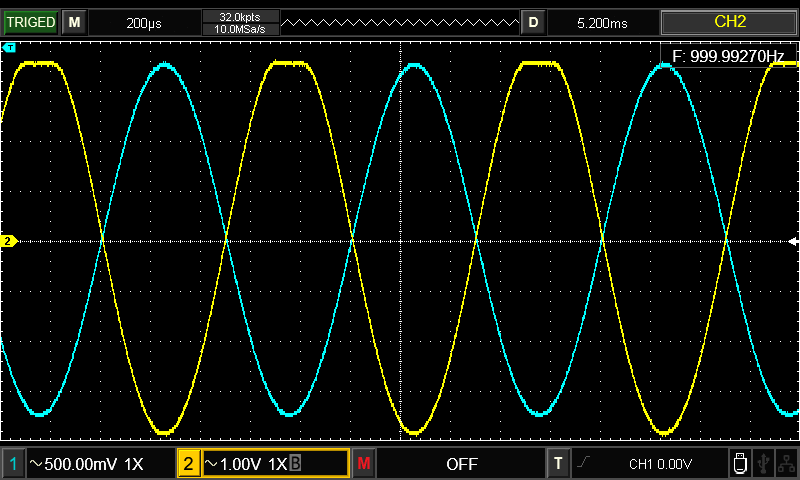
\includegraphics[height=5cm\textwidth]{distorsionsRLsCE.png}
        \caption{$V_g$ (curva azul) necesario para distorsión de $V_o$ (curva amarilla)}
        \label{fig:vdis1}
    \end{figure}

    \begin{table}[h!]
        \centering
        \caption{Tensiones pico-pico referidas a la figura \ref{fig:vdis1}}
        \label{tab:vdis1}
        \begin{tabular}{|c|c|} \hline
            $V_i [V_{PP}]$  &   $V_o [V_{PP}]$  \\ \hline
            3.6 \pm 0.1     &   7.4 \pm 0.2    \\ \hline
        \end{tabular}
    \end{table}

    \begin{figure}
        \centering
        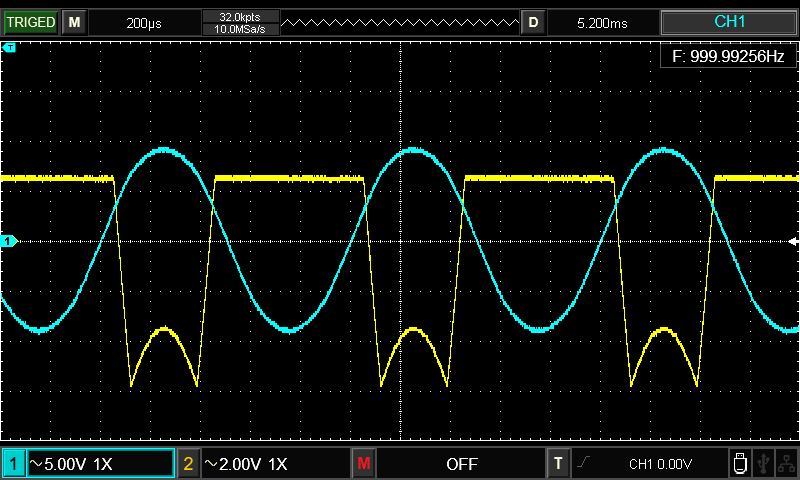
\includegraphics[height=5cm\textwidth]{MAXsRLsCE.png}
        \caption{señal de salida $V_o$ (curva amarilla) con máxima $V.g = 20 V_PP$ (curva azul)}
        \label{fig:vmax1}
    \end{figure}

    \begin{table}[h!]
        \centering
        \caption{Tensiones pico-pico referidas a la figura \ref{fig:vmax1}}
        \label{tab:vmax1}
        \begin{tabular}{|c|c|} \hline
            $V_i [V_{PP}]$  &   $V_o [V_{PP}]$  \\ \hline
            20 \pm 1     &   8.4 \pm 0.4    \\ \hline
        \end{tabular}
    \end{table}

    \newpage

    \subsection{Prueba de laboratorio \ref{lab2} con RL sin CE}

    \begin{figure}
        \centering
        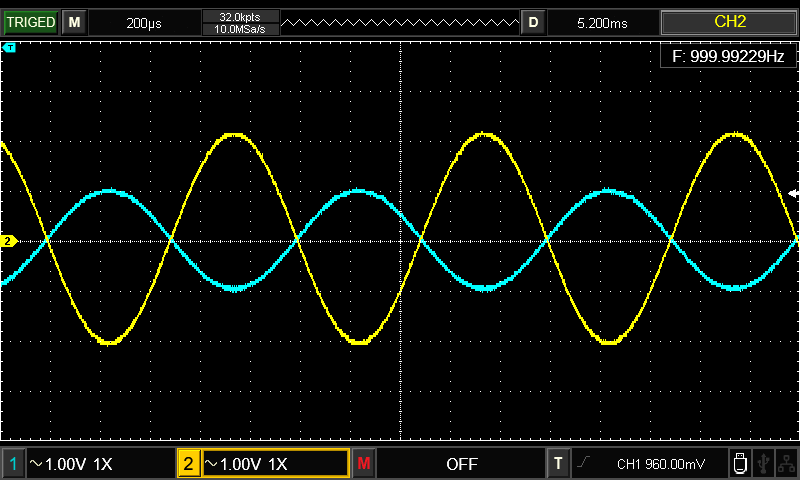
\includegraphics[height=5cm\textwidth]{ViocRLsCE.png}
        \caption{Señal de entrada $V_i$ (curva azul) y componete AC de señal de salida $V_o$ (curva amarilla)}
        \label{fig:vio2}
    \end{figure}

    Basandose en las señales de la figura \ref{fig:vio2} se recopilaron los siguientes datos

    \begin{table}[h!]
        \centering
        \caption{Tensiones pico-pico de entrada y salida con RL sin CE}
        \label{tab:vio2}
        \begin{tabular}{|c|c|c|} \hline
            $V_i  [V_{PP}]$  &  $V_o  [V_{PP}]$   &  $V_{Pmax} [V]$\\ \hline
            2.0 ± 0.2        &     -4.0 ± 0.2     &  10.0 \pm 1.2 \\ \hline
        \end{tabular}
    \end{table}

    {\bf Observación.} Para $V_{Pmax}$ se tomó el $V_o [V_P]$ en semiciclo positivo y se le sumó el escalón de la componente DC representada en la figura \ref{fig:vc}.

    Se calcularon las ganancias de tensión experimentales con la ecuacion \eqref{eqAv} referida en los anexos. Por otra parte, la ganancia teorica queda señalada en la tabla \ref{tab:rteo} en la sección de Cálculos prévios.

    \begin{table}[h!]
        \centering
        \caption{Ganancia relacionada al amplificador de la figura \ref{fig:circuito} con RL sin CE}
        \label{tab:av2}
        \begin{tabular}{|c|c|c|} \hline
            $Av_{exp} \; [V/V]$  &  $Av_{teo} \; [V/V]$  & Desviación [\%] \\ \hline
            -2.00 ± 0.22         &       -2.11              & 5   \\ \hline
        \end{tabular}
    \end{table}

    \subsubsection{Implementando resistencias patrón ($R_P$) para cálculo de impeancias experimentales}

    Basandose en el modelo lineal de amplificador de la figura \ref{fig:rp} en la sección de anexos.

    \begin{table}[h!]
        \centering
        \caption{Resistencias patrones en circuito de la figura \ref{fig:circuito} con RL sin CE}
        \label{tab:rp2}
        \begin{tabular}{|c|c|} \hline
            $R_{P_{Ri}}$          &  $R_{P_{Ro}}$  \\ \hline
            $15k\Omega \pm 10\%$  &  $470\Omega \pm 10\%$    \\ \hline
        \end{tabular}
    \end{table}

    \newpage

    \begin{figure}[h!]
        \centering
        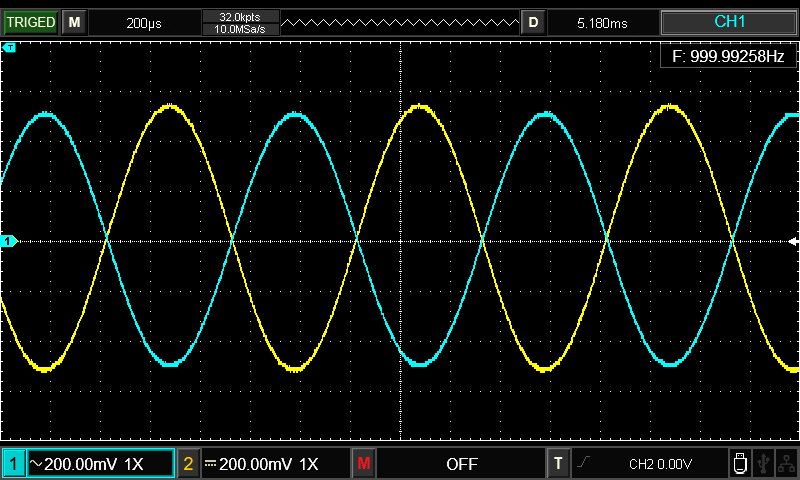
\includegraphics[height=5cm\textwidth]{RPcRLsCE.png}
        \caption{Señal $V_{R_{PRi}}$ (curva azul) y componete AC de señal de salida $V_{occ}$ (curva amarilla)}
        \label{fig:vrp2}
    \end{figure}

    De la figura \ref{fig:vrp2} se establecen los siguientes voltajes pico-pico

    \begin{table}[h!]
        \centering
        \caption{Tensiones pico-pico del terminal de las resistencias patrones asociadas a la figura \ref{fig:vrp2}}
        \label{tab:vrp2}
        \begin{tabular}{|c|c|} \hline
            $V_{R_i} [V_{PP}]$  &   $V_{occ} [V_{PP}]$  \\ \hline
            0.96 ± 0.04         &   1.04 ± 0.04    \\ \hline
        \end{tabular}
    \end{table}

    Sabiendo que $V_o = V_{osc}$ y utilizando las ecuaciones \eqref{eqri} y \eqref{eqro} de la sección de los anexos

    \begin{table}[h!]
        \centering
        \caption{Impedancia de entrada en circuito de la figura \ref{fig:circuito} con RL sin CE}
        \label{tab:rpi2}
        \begin{tabular}{|c|c|c|} \hline
            $R_{i_{EXP}} [k\Omega]$  &   $R_{i_{TEO}} [k\Omega]$ & Desviación [\%]  \\ \hline
            13.85         &   15.7   & 12 \\ \hline
        \end{tabular}
    \end{table}

    \begin{table}[h!]
        \centering
        \caption{Impedancias de salida en circuito de la figura \ref{fig:circuito} con RL sin CE}
        \label{tab:rpo2}
        \begin{tabular}{|c|c|c|} \hline
            $R_{o_{EXP}} [\Omega]$  &   $R_{o_{TEO}} [\Omega]$ & Desviación [\%]  \\ \hline
            1338         &   485   & 176 \\ \hline
        \end{tabular}
    \end{table}

    \newpage

    \begin{figure}[h!]
        \centering
        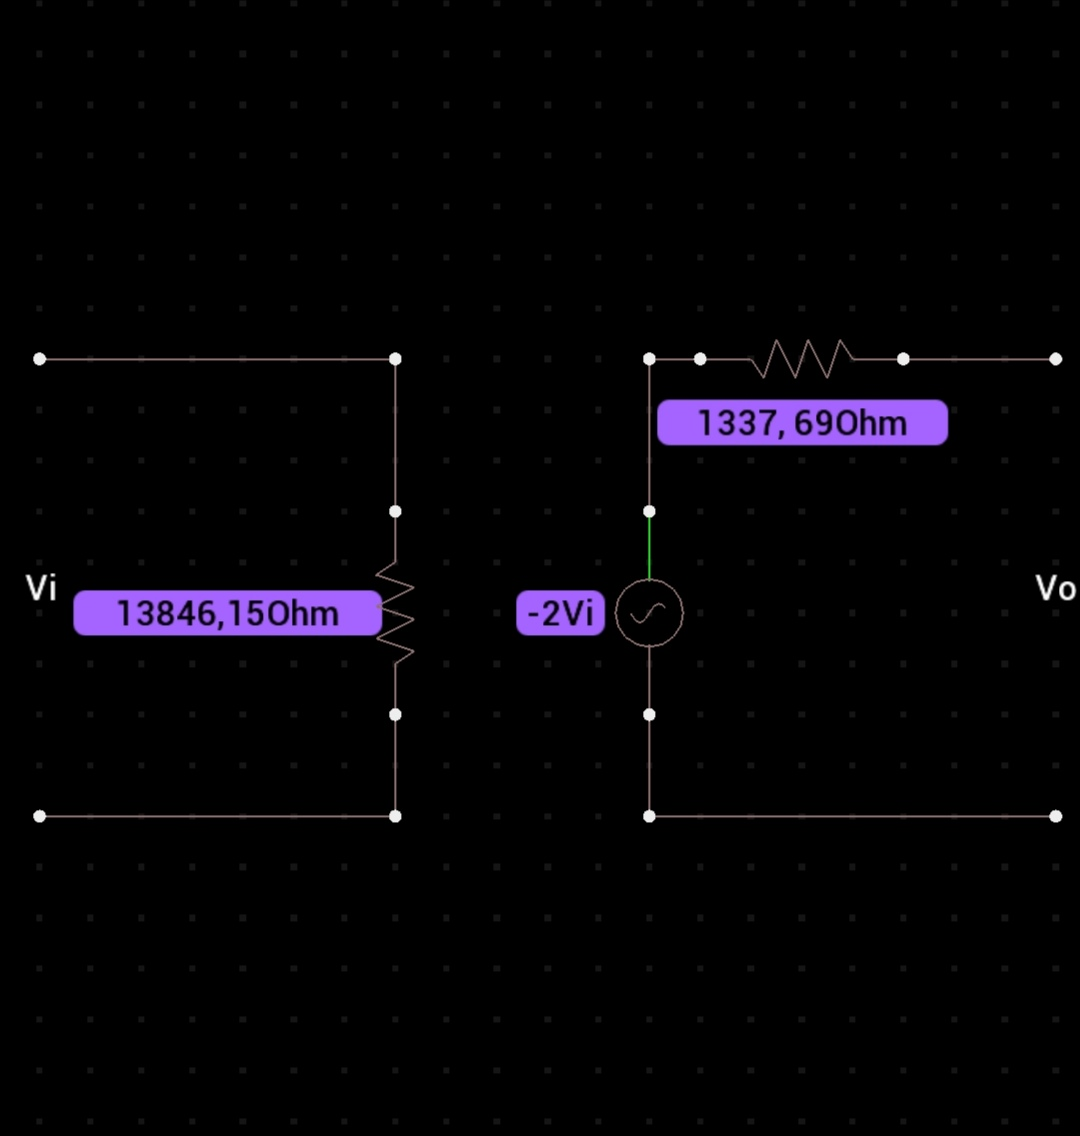
\includegraphics[height=5cm\textwidth]{ma2.jpg}
        \caption{Modelo lineal de amplificador de tensión para circuito de la figura \ref{fig:circuito} con RL sin CE}
        \label{fig:ma2}
    \end{figure}

    \subsubsection{Variacion de amplitud de la señal $V_g$}

    \begin{figure}[h!]
        \centering
        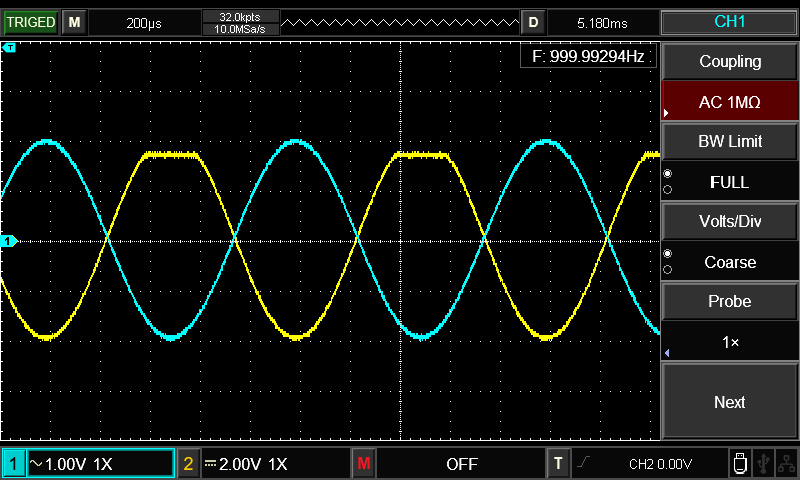
\includegraphics[height=5cm\textwidth]{distorsioncRLsCE.png}
        \caption{$V_g$ (curva azul) necesario para distorsión de $V_o$ (curva amarilla)}
        \label{fig:vdis2}
    \end{figure}

    \begin{table}[h!]
        \centering
        \caption{Tensiones pico-pico referidas a la figura \ref{fig:vdis2}}
        \label{tab:vdis2}
        \begin{tabular}{|c|c|} \hline
            $V_i [V_{PP}]$  &   $V_o [V_{PP}]$  \\ \hline
            4.0 \pm 0.2     &   7.6 \pm 0.4    \\ \hline
        \end{tabular}
    \end{table}

    \newpage

    \begin{figure}[h!]
        \centering
        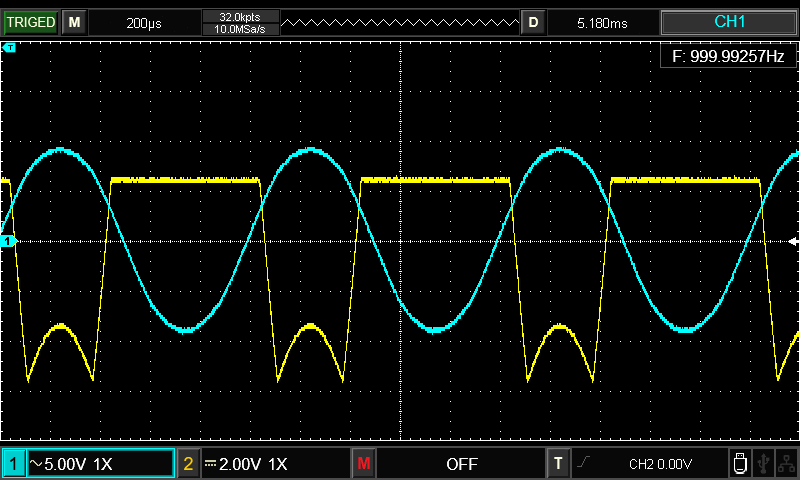
\includegraphics[height=5cm\textwidth]{MAXcRLsCE.png}
        \caption{señal de salida $V_o$ (curva amarilla) con máxima $V.g = 20 V_PP$ (curva azul)}
        \label{fig:vmax2}
    \end{figure}

    \begin{table}[h!]
        \centering
        \caption{Tensiones pico-pico referidas a la figura \ref{fig:vmax2}}
        \label{tab:vmax2}
        \begin{tabular}{|c|c|} \hline
            $V_i [V_{PP}]$  &   $V_o [V_{PP}]$  \\ \hline
            20 \pm 1     &   8.0 \pm 0.4    \\ \hline
        \end{tabular}
    \end{table}

    \subsection{Prueba de laboratorio \ref{lab3} sin RL, con CE}

    \begin{figure}
        \centering
        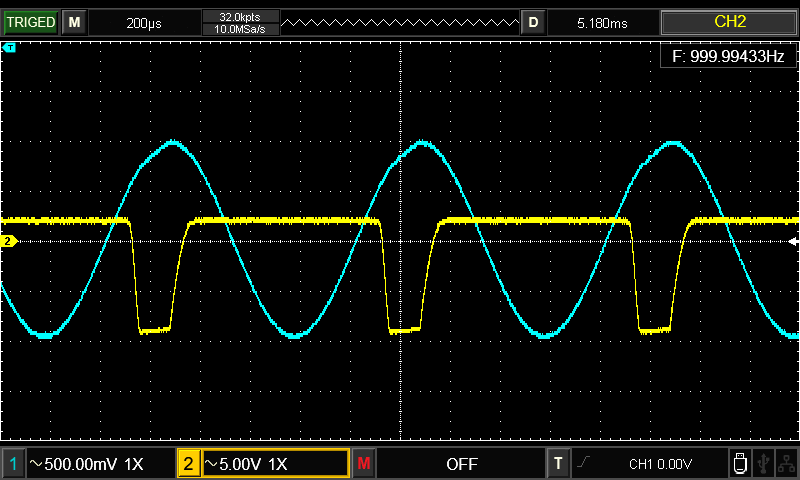
\includegraphics[height=5cm\textwidth]{ViosRLcCE.png}
        \caption{Señal de entrada $V_i$ (curva azul) y componete AC de señal de salida $V_o$ (curva amarilla)}
        \label{fig:vio3}
    \end{figure}

    Basandose en las señales de la figura \ref{fig:vio3} se recopilaron los siguientes datos

    \begin{table}[h!]
        \centering
        \caption{Tensiones pico-pico de entrada y salida sin RL, con CE}
        \label{tab:vio3}
        \begin{tabular}{|c|c|c|} \hline
            $V_i  [V_{PP}]$  &  $V_o  [V_{PP}]$   &  $V_{Pmax} [V]$\\ \hline
            2.0 ± 0.1        &     -11 ± 1     &  10 \pm 2 \\ \hline
        \end{tabular}
    \end{table}

    {\bf Observación.} Para $V_{Pmax}$ se tomó el $V_o [V_P]$ en semiciclo positivo y se le sumó el escalón de la componente DC representada en la figura \ref{fig:vc}.

    \newpage

    Se calcularon las ganancias de tensión experimentales con la ecuacion \eqref{eqAv} referida en los anexos. Por otra parte, la ganancia teorica queda señalada en la tabla \ref{tab:rteo} en la sección de Cálculos prévios.

    \begin{table}[h!]
        \centering
        \caption{Ganancia relacionada al amplificador de la figura \ref{fig:circuito} sin RL, con CE}
        \label{tab:av3}
        \begin{tabular}{|c|c|c|} \hline
            $Av_{exp} \; [V/V]$  &  $Av_{teo} \; [V/V]$  & Desviación [\%] \\ \hline
            -5.50 ± 0.57         &       -17.85          & 69   \\ \hline
        \end{tabular}
    \end{table}

    \subsubsection{Implementando resistencias patrón ($R_P$) para cálculo de impeancias experimentales}

    Basandose en el modelo lineal de amplificador de la figura \ref{fig:rp} en la sección de anexos.

    \begin{table}[h!]
        \centering
        \caption{Resistencias patrones en circuito de la figura \ref{fig:circuito} sin RL, con CE}
        \label{tab:rp3}
        \begin{tabular}{|c|c|} \hline
            $R_{P_{Ri}}$          &  $R_{P_{Ro}}$  \\ \hline
            $5.1k\Omega \pm 10\%$  &  $470\Omega \pm 10\%$    \\ \hline
        \end{tabular}
    \end{table}

    \begin{figure}[h!]
        \centering
        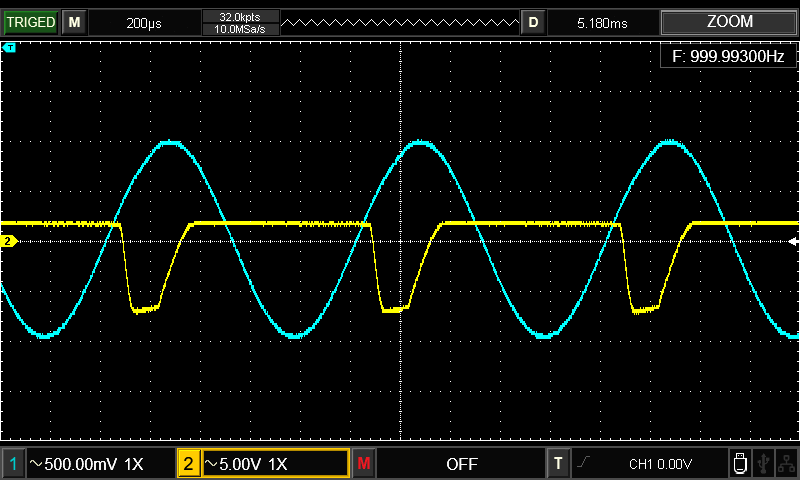
\includegraphics[height=5cm\textwidth]{RPsRLcCE.png}
        \caption{Señal $V_{R_{PRi}}$ (curva azul) y componete AC de señal de salida $V_{occ}$ (curva amarilla)}
        \label{fig:vrp3}
    \end{figure}

    De la figura \ref{fig:vrp3} se establecen los siguientes voltajes pico-pico

    \begin{table}[h!]
        \centering
        \caption{Tensiones pico-pico del terminal de las resistencias patrones asociadas a la figura \ref{fig:vrp3}}
        \label{tab:vrp3}
        \begin{tabular}{|c|c|} \hline
            $V_{R_i} [V_{PP}]$  &   $V_{occ} [V_{PP}]$  \\ \hline
            2.0 ± 0.1         &   11 ± 1    \\ \hline
        \end{tabular}
    \end{table}

    \newpage

    Sabiendo que $V_o = V_{osc}$ y utilizando las ecuaciones \eqref{eqri} y \eqref{eqro} de la sección de los anexos

    \begin{table}[h!]
        \centering
        \caption{Impedancia de entrada en circuito de la figura \ref{fig:circuito} sin RL, con CE}
        \label{tab:rpi3}
        \begin{tabular}{|c|c|c|} \hline
            $R_{i_{EXP}} [k\Omega]$  &   $R_{i_{TEO}} [k\Omega]$ & Desviación [\%]  \\ \hline
            \infty         &   4.2   & \infty \\ \hline
        \end{tabular}
    \end{table}

    \begin{table}[h!]
        \centering
        \caption{Impedancias de salida en circuito de la figura \ref{fig:circuito} sin RL, con CE}
        \label{tab:rpo3}
        \begin{tabular}{|c|c|c|} \hline
            $R_{o_{EXP}} [\Omega]$  &   $R_{o_{TEO}} [\Omega]$ & Desviación [\%]  \\ \hline
            104         &   510   & 80 \\ \hline
        \end{tabular}
    \end{table}

    \begin{figure}
        \centering
        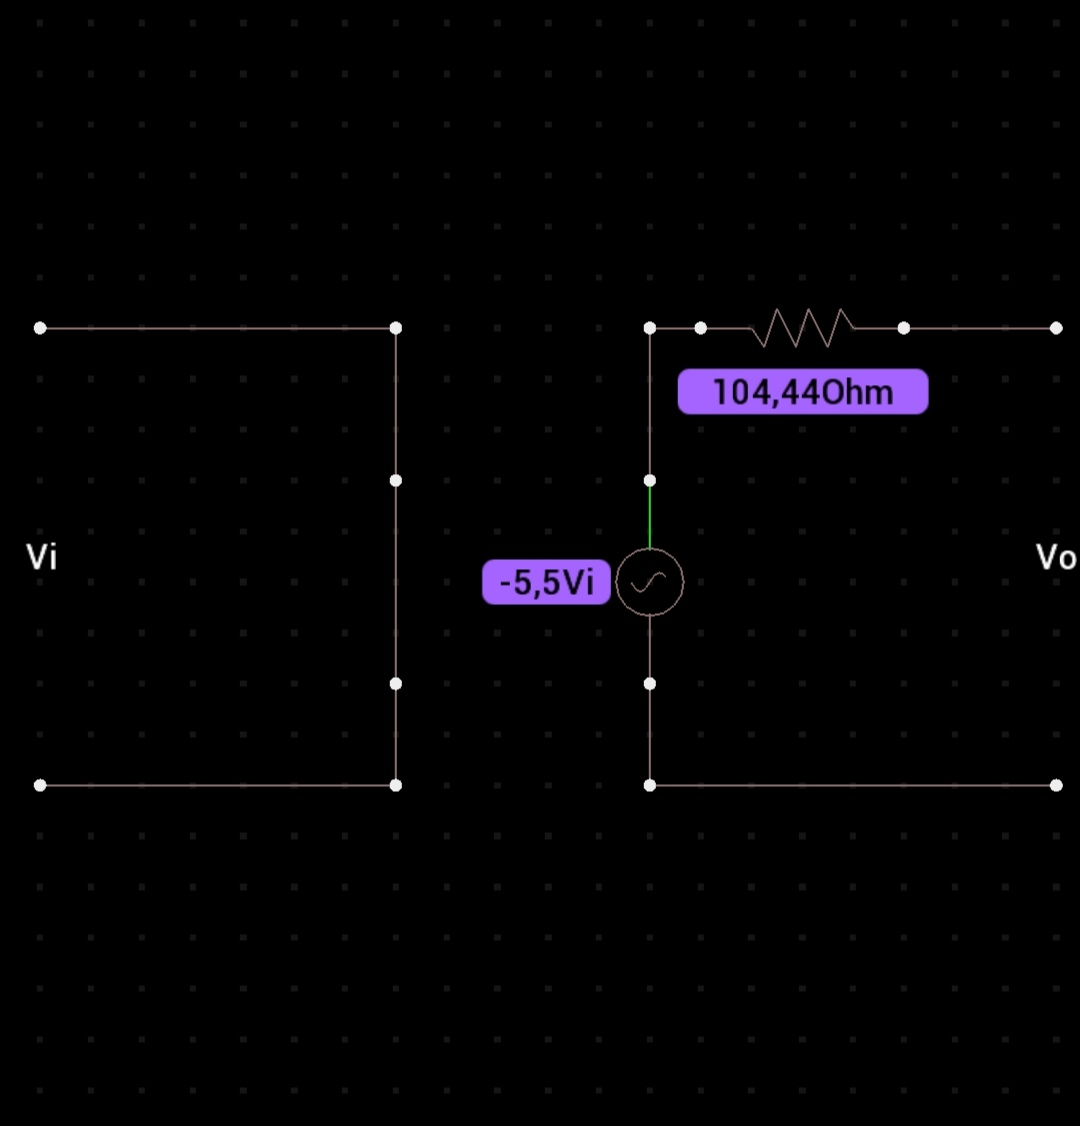
\includegraphics[height=5cm\textwidth]{ma3.jpg}
        \caption{Modelo lineal de amplificador de tensión para circuito de la figura \ref{fig:circuito} sin RL, con CE}
        \label{fig:ma3}
    \end{figure}

    \newpage

    \subsubsection{Variacion de amplitud de la señal $V_g$}

    \begin{figure}
        \centering
        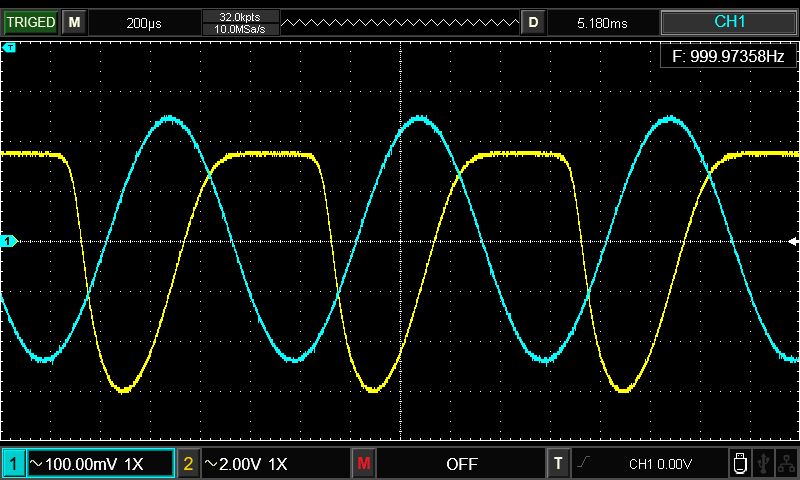
\includegraphics[height=5cm\textwidth]{05distorsionsRLcCE.png}
        \caption{$V_g$ (curva azul), con distorsión de $V_o$ (curva amarilla)}
        \label{fig:vdis3}
    \end{figure}

    \begin{table}[h!]
        \centering
        \caption{Tensiones pico-pico referidas a la figura \ref{fig:vdis3}}
        \label{tab:vdis3}
        \begin{tabular}{|c|c|} \hline
            $V_i [V_{PP}]$  &   $V_o [V_{PP}]$  \\ \hline
            0.48 \pm 0.02     &   9.6 \pm 0.4    \\ \hline
        \end{tabular}
    \end{table}

    \begin{figure}
        \centering
        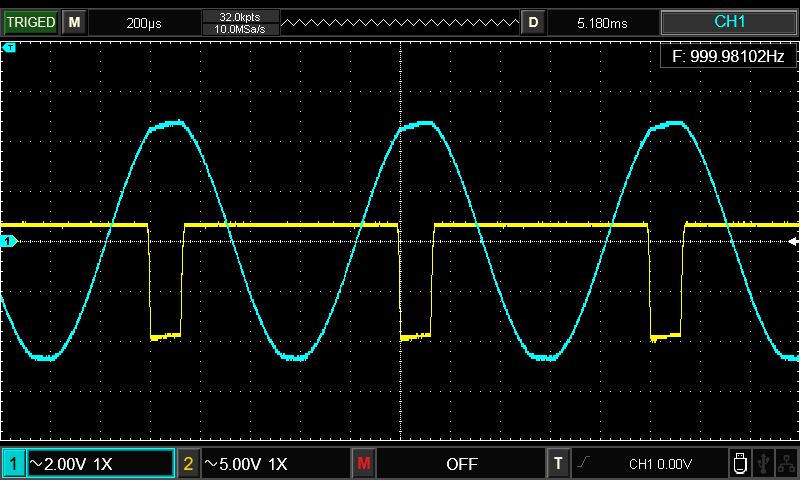
\includegraphics[height=5cm\textwidth]{MAXsRLcCE.png}
        \caption{señal de salida $V_o$ (curva amarilla) con máxima $V.g = 10 V_PP$ (curva azul)}
        \label{fig:vmax3}
    \end{figure}

    \begin{table}[h!]
        \centering
        \caption{Tensiones pico-pico referidas a la figura \ref{fig:vmax3}}
        \label{tab:vmax3}
        \begin{tabular}{|c|c|} \hline
            $V_i [V_{PP}]$  &   $V_o [V_{PP}]$  \\ \hline
            9.6 \pm 0.4     &   12 \pm 1    \\ \hline
        \end{tabular}
    \end{table}

    \newpage

    \subsection{Prueba de laboratorio \ref{lab4} con RL y CE}

    \begin{figure}
        \centering
        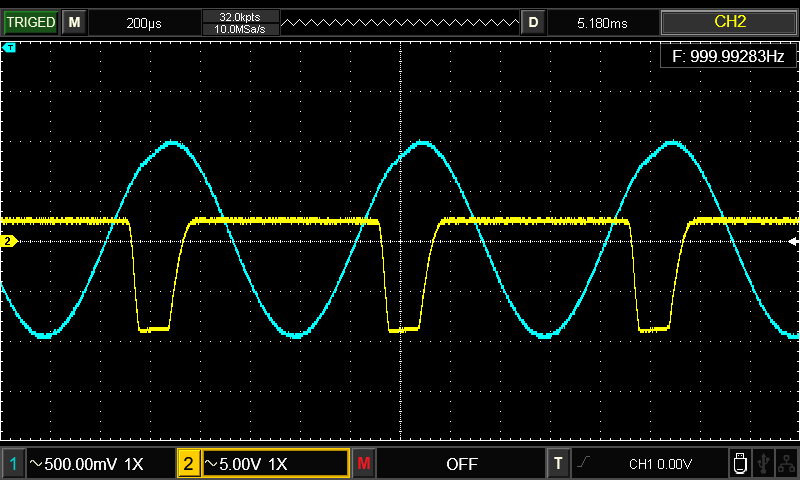
\includegraphics[height=5cm\textwidth]{ViocRLcCE.png}
        \caption{Señal de entrada $V_i$ (curva azul) y componete AC de señal de salida $V_o$ (curva amarilla)}
        \label{fig:vio4}
    \end{figure}

    Basandose en las señales de la figura \ref{fig:vio4} se recopilaron los siguientes datos

    \begin{table}[h!]
        \centering
        \caption{Tensiones pico-pico de entrada y salida con RL y CE}
        \label{tab:vio4}
        \begin{tabular}{|c|c|c|} \hline
            $V_i  [V_{PP}]$  &  $V_o  [V_{PP}]$   &  $V_{Pmax} [V]$\\ \hline
            2.0 ± 0.1        &     -11 ± 1     &  10 \pm 2 \\ \hline
        \end{tabular}
    \end{table}

    {\bf Observación.} Para $V_{Pmax}$ se tomó el $V_o [V_P]$ en semiciclo positivo y se le sumó el escalón de la componente DC representada en la figura \ref{fig:vc}.

    Se calcularon las ganancias de tensión experimentales con la ecuacion \eqref{eqAv} referida en los anexos. Por otra parte, la ganancia teorica queda señalada en la tabla \ref{tab:rteo} en la sección de Cálculos prévios.

    \begin{table}[h!]
        \centering
        \caption{Ganancia relacionada al amplificador de la figura \ref{fig:circuito} con RL y CE}
        \label{tab:av4}
        \begin{tabular}{|c|c|c|} \hline
            $Av_{exp} \; [V/V]$  &  $Av_{teo} \; [V/V]$  & Desviación [\%] \\ \hline
            -5.50 ± 0.57         &       -16.98          & 68   \\ \hline
        \end{tabular}
    \end{table}

    \subsubsection{Implementando resistencias patrón ($R_P$) para cálculo de impeancias experimentales}

    Basandose en el modelo lineal de amplificador de la figura \ref{fig:rp} en la sección de anexos.

    \begin{table}[h!]
        \centering
        \caption{Resistencias patrones en circuito de la figura \ref{fig:circuito} con RL y CE}
        \label{tab:rp4}
        \begin{tabular}{|c|c|} \hline
            $R_{P_{Ri}}$          &  $R_{P_{Ro}}$  \\ \hline
            $5.1k\Omega \pm 10\%$  &  $470\Omega \pm 10\%$    \\ \hline
        \end{tabular}
    \end{table}

    \newpage

    \begin{figure}[h!]
        \centering
        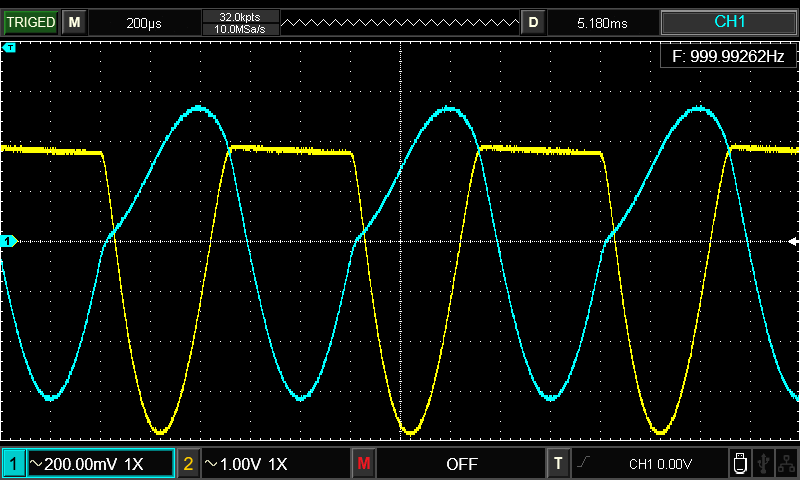
\includegraphics[height=5cm\textwidth]{RPcRLcCE.png}
        \caption{Señal $V_{R_{PRi}}$ (curva azul) y componete AC de señal de salida $V_{occ}$ (curva amarilla)}
        \label{fig:vrp4}
    \end{figure}

    De la figura \ref{fig:vrp4} se establecen los siguientes voltajes pico-pico

    \begin{table}[h!]
        \centering
        \caption{Tensiones pico-pico del terminal de las resistencias patrones asociadas a la figura \ref{fig:vrp4}}
        \label{tab:vrp4}
        \begin{tabular}{|c|c|} \hline
            $V_{R_i} [V_{PP}]$  &   $V_{occ} [V_{PP}]$  \\ \hline
            1.12 ± 0.04         &   5.6 ± 0.2    \\ \hline
        \end{tabular}
    \end{table}

    Sabiendo que $V_o = V_{osc}$ y utilizando las ecuaciones \eqref{eqri} y \eqref{eqro} de la sección de los anexos

    \begin{table}[h!]
        \centering
        \caption{Impedancia de entrada en circuito de la figura \ref{fig:circuito} con RL y CE}
        \label{tab:rpi4}
        \begin{tabular}{|c|c|c|} \hline
            $R_{i_{EXP}} [k\Omega]$  &   $R_{i_{TEO}} [k\Omega]$ & Desviación [\%]  \\ \hline
            6.49         &   4.2   & 55 \\ \hline
        \end{tabular}
    \end{table}

    \begin{table}[h!]
        \centering
        \caption{Impedancias de salida en circuito de la figura \ref{fig:circuito} con RL y CE}
        \label{tab:rpo4}
        \begin{tabular}{|c|c|c|} \hline
            $R_{o_{EXP}} [\Omega]$  &   $R_{o_{TEO}} [\Omega]$ & Desviación [\%]  \\ \hline
            453         &   485   & 7 \\ \hline
        \end{tabular}
    \end{table}

    \newpage

    \begin{figure}[h!]
        \centering
        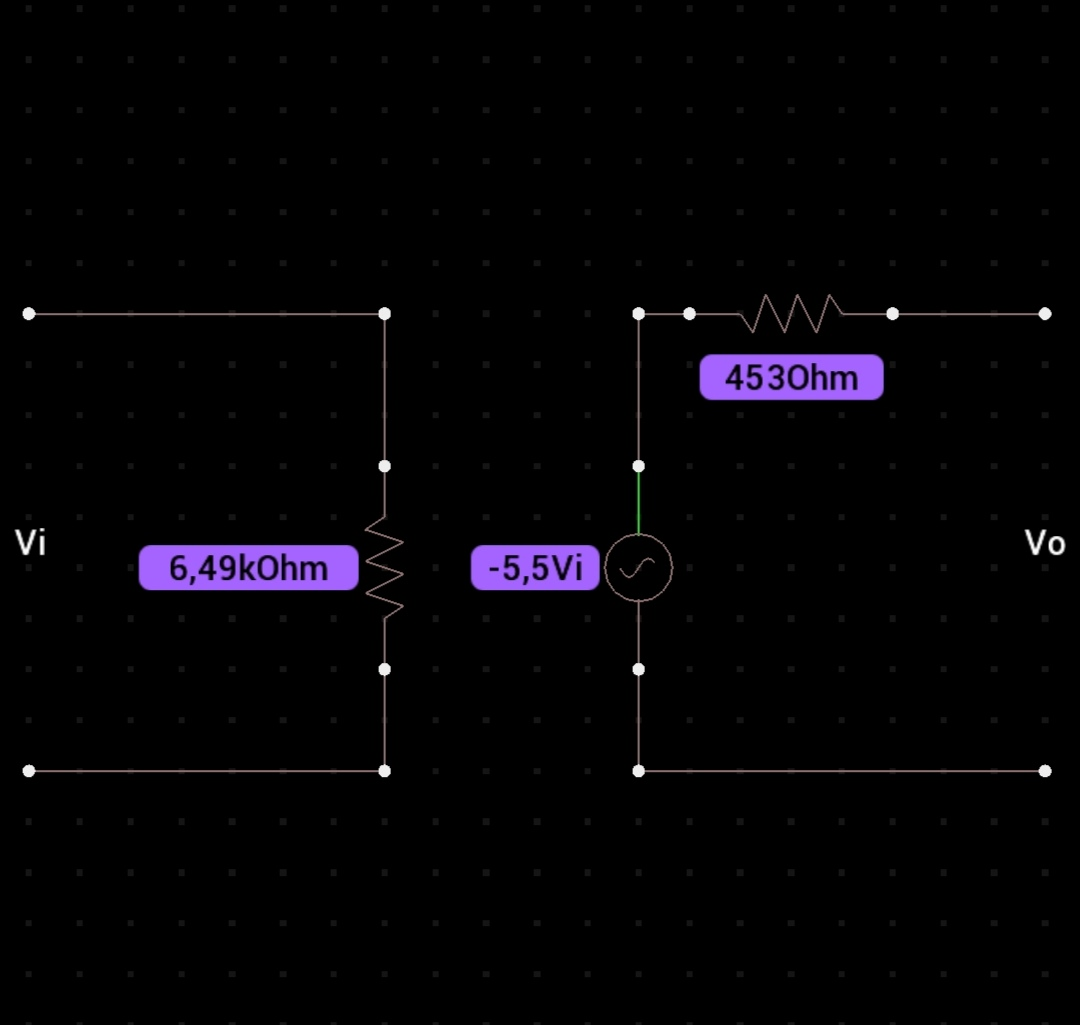
\includegraphics[height=5cm\textwidth]{ma4.jpg}
        \caption{Modelo lineal de amplificador de tensión para circuito de la figura \ref{fig:circuito} con RL y CE}
        \label{fig:ma4}
    \end{figure}

    \subsubsection{Variacion de amplitud de la señal $V_g$}

    \begin{figure}[h!]
        \centering
        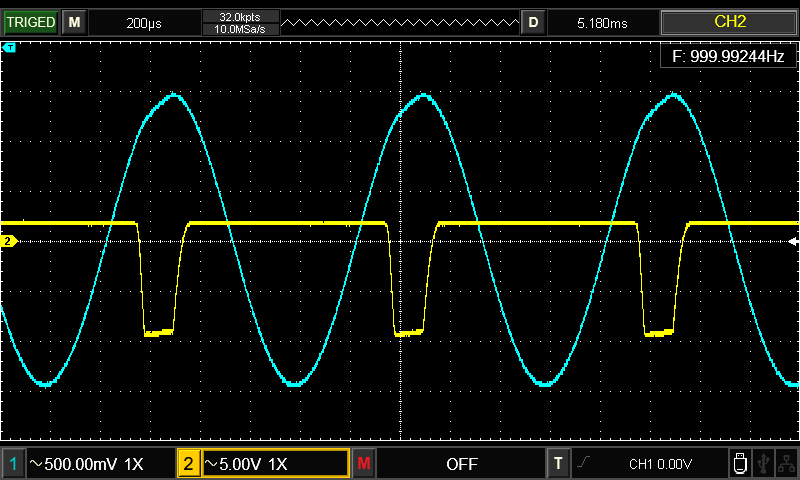
\includegraphics[height=5cm\textwidth]{3distorsioncRLcCE.png}
        \caption{$V_g$ (curva azul), con distorsión de $V_o$ (curva amarilla)}
        \label{fig:vdis4}
    \end{figure}

    \begin{table}[h!]
        \centering
        \caption{Tensiones pico-pico referidas a la figura \ref{fig:vdis4}}
        \label{tab:vdis4}
        \begin{tabular}{|c|c|} \hline
            $V_i [V_{PP}]$  &   $V_o [V_{PP}]$  \\ \hline
            3.0 \pm 0.1     &   11 \pm 1    \\ \hline
        \end{tabular}
    \end{table}

    \newpage

    \begin{figure}[h!]
        \centering
        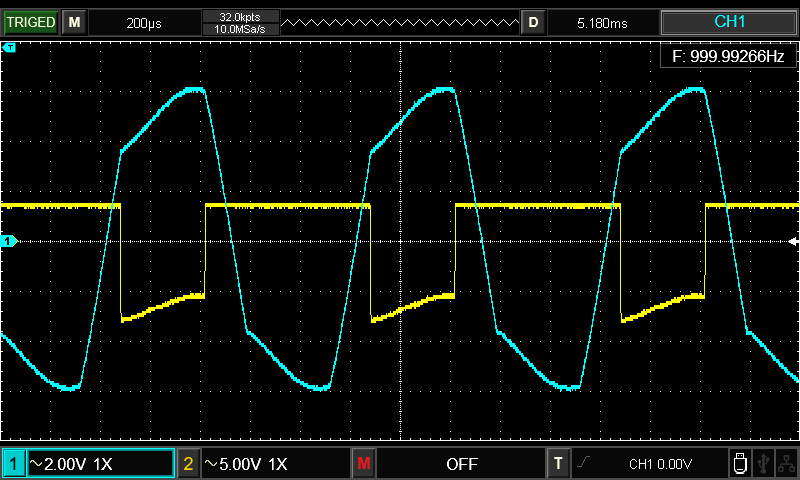
\includegraphics[height=5cm\textwidth]{MAXcRLcCE.png}
        \caption{señal de salida $V_o$ (curva amarilla) con máxima $V.g = 10 V_PP$ (curva azul)}
        \label{fig:vmax4}
    \end{figure}

    \begin{table}[h!]
        \centering
        \caption{Tensiones pico-pico referidas a la figura \ref{fig:vmax4}}
        \label{tab:vmax4}
        \begin{tabular}{|c|c|} \hline
            $V_i [V_{PP}]$  &   $V_o [V_{PP}]$  \\ \hline
            12.0 \pm 0.4     &   12 \pm 1    \\ \hline
        \end{tabular}
    \end{table}

    \newpage

    \section{Análisis de Resultados}

    Se sabe tanto por la tabla experimental \ref{tab:Q} como por el cáculo teórico \eqref{eqQ} que el transistor está operando en la zona activa, pues los valores de $V_{CE}$ rodean entre los 6V y 8V, además $I_C$ es razonable respectivamente, y al compararlos esnotable que el valor de la corriente y del voltaje si se aproxima al valor calculado; la particularidad del valor de $h_{FE}$ para cada transistor altera de forma apreciable los cálculos.

    Es de gran importancia considerar que todas las señales AC referentes a las mediciones realizadas en la salida $V_o$ poseen una componente DC debido al punto estático de operacion; este hecho se aprecia en la Figura \ref{fig:vo}, donde la componente AC hace que el punto de operacion estático se mantenga oscilando alrededor del escalón DC de $8V$.

    Para las pruebas de laboratorio \ref{lab1} y \ref{lab2} las ganancias experimentales expresadas en las tablas \ref{tab:av1} y \ref{tab:av2} demuestran una desviación porcentual menor o igual al $5\%$, lo que implica un comportamiento estable en la relación de entrada y salida del amplificador, sin la presencia del capacitor CE. Sin embargo este comportamiento comienza a cambiar al aumentar la tensión pico-pico de la señal de entrada a una tensión mayor de $3.6V_PP$, donde como se puede observar en la Figura \ref{fig:vdis1} que la señal no completa totalmente el semiciclo positivo, esto debido a que el punto de operación entra en zona de corte, ya que alcanza una tension pico máxima igual a la tensión de alimentación de $12V$ que no puede sobrepasar. Por consiguiente, al aumentar la señal de entrada con un valor aproximado a la tensión de alimentación, como el caso de la Figura \ref{fig:vmax1}, se produce una tensión negativa en la entrada que polariza la unión base-emisor directamente y, por tanto, lleva el punto de operacion a la zona de saturación en los semiciclos negativos. Por otra parte, las tablas \ref{tab:rpi1} y \ref{tab:rpi2} muestran una alta correlación con los valores teorico en la tabla \ref{tab:rteo} para las impedancias de entrada debido a su baja desviación, que, sin importar si el amplificador posee RL o no, se puede considerar un $R_i = 15.7K\Omega$; caso que no sucede con la impedancia de salida expresada en la tablas \ref{tab:rpo1} y \ref{tab:rpo2} que posee una alta desviación respecto al valor teorico.

    Al colocar el condensador CE al circuito de la figura \ref{fig:circuito} es notable en las tablas \ref{tab:av3} y \ref{tab:av4} que la ganancia aumenta, como es de esperarse según los cálculos prévios, sin embargo, existe una alta desviación. Esto se explica por el hecho de entrar en la zona de corte al llegar a los 12V, según lo que se dijo en el párrafo anterior; produciendo así según las figuras \ref{fig:vio3} y \ref{fig:vio4} una distorsión en la salida $V_o$ con la señal $V_i = 2V_{PP}$ predeterminada, sin alteración por RL. Al disminuir la amplitud en la figura \ref{fig:vdis3} se pudo apreciar mejor el efecto de mayor ganancia que produce la implementación de CE tomando en consideracion los datos de la tabla \ref{tab:vdis3}. Cabe mencionar que las resistencias de entrada y salida relacionadas con la prueba de laboratorio \ref{lab3} tendieron a valores extremos, donde $R_i$ puede ser considerado un componente abierto y $R_o$ uno cerrrado, optimizando en este caso el efecto que produce $V_i$ cuando el amplificador no posee carga RL. Entonces para la prueba \ref{lab4} donde las resistencias de entrada y salida poseen bajas desviaciones según las tablas \ref{tab:rpi3} y \ref{tab:rpi4}; y la ganancia es mayor, se puede considerar el modelo circuital lineal de la figura \ref{fig:ma4} como apropiado para señales de amplitud baja.

    Cabe mencionar que en los casos estudiados en este informe no se aprecia un cambio significativo en la frecuencia de la onda de salida con respecto a la de entrada.

    \newpage

    \section{Conclusiones y Recomendaciones}

    En este informe se ha estudiado el comportamiento dinámico de un amplificador básico de tensión en configuración de emisor común. El objetivo era analizar el efecto sobre la ganancia de tensión al colocar un condensador de desacoplo en paralelo con la resistencia de emisor, primero sin carga en el amplificador y luego con carga.

    Con los resultados obtenidos se concluye que el efecto de conectar un condensador de desacoplo a un amplificador BJT es que se mejora la ganancia de voltaje del circuito, el condensador se usa para eliminar el ruido o las señales de CA que puedan estar presentes en la fuente de alimentación del circuito. Estas señales pueden interferir con el funcionamiento del amplificador y causar distorsión o inestabilidad. El condensador de desacoplo actúa como un filtro que conduce las señales de CA a tierra, dejando pasar solamente la señal de CD. De esta forma, se mejora la calidad y la precisión de la señal amplificada.
    
    Por otro lado, el efecto de conectar una carga en configuración de emisor común a un amplificador BJT es que se reduce la ganancia de voltaje del circuito. Esto se debe a que la carga se suma a la resistencia del colector RC, disminuyendo la caída de voltaje entre el colector y el emisor, Sin embargo, se puede observar en los datos experimentales y teóricos que dicha disminución es pequeña, lo suficientemente pequeña para poder despreciarla para ciertas aplicaciones.
    
    Por último se observó que las impedancias de entrada y salida y la ganancia calculadas pueden ser muy distintas a las medidas experimentalmente, pero esto puede ser por una mala elección de los parámetros híbridos que influyen en el cálculo de esos valores. La medición para hallar la ganancia y las impedancias es fácil y el método para obtener los valores de las ganancias y las impedancias es muy simple, así que podríamos concluir que si se tienen o conocen los parámetors correctos es mucho mejor hallar las ganancias y las impedancias experimentalmente.

    \newpage

    \section{Bibliografía}

    \begin{itemize}
        \item Sedra Adel. “Circuitos Microelectr´onicos”. En: OXFORD University Press 4 (2002).
        \item Panayotis Tremante. "Método resistencia patrón". En (2024). Documento digital.
    \end{itemize}
    
    \printbibliography

    \newpage

    \section{Anexos}

    \subsection{Cálculo del punto de operación}

    Para los valores $V_{CE}$ y $I_C$ de la tabla \ref{tab:Q} se realizaron los siguientes cálculos:

    Sabiendo que $V_{CC} = 12 \pm 1 [V]$

    \begin{equation}
        V_{CE} = V_C - V_E
        \label{Qeq1}
    \end{equation}

    \begin{equation}
        I_C = \frac{V_{CC} - V_C}{R_C}
        \label{Qeq2}
    \end{equation}

    Para el cálculo de sus respectivas incertidumbres:

    \begin{equation}
        \Delta V_{CE} = \Delta V_C + \Delta V_E
        \label{Qeq3}
    \end{equation}

    \begin{equation}
        \begin{split}
            \Delta I_C & = \left | \frac{\partial I_C}{\partial V_{CC}} \right | \Delta V_{CC} + \left | \frac{\partial I_C}{\partial V_C} \right | \Delta V_C + \left | \frac{\partial I_C}{\partial R_C} \right | \Delta R_C \\
            & = {1 \over R_C} \Delta V_{CC} + {1 \over R_C} \Delta V_C + \frac{V_{CC}-V_C}{R_C^2} \Delta R_C
        \end{split}
        \label{Qeq4}
    \end{equation}

    \subsection{Cálculo de ganancia}

    Para las tablas \ref{tab:av1}, \ref{tab:av2}, \ref{tab:av3} y \ref{tab:av4} se calculó la ganancia a través de la siguiente ecuación, basandose en la ecuación\eqref{ganancia},

    \begin{equation} \label{eqAv}
        A_V = {V_o \over V_i} \pm {V_o \over V_i}\sqrt{\left( {\Delta V_o \over V_o} \right)^2 + \left( {\Delta V_i \over V_i} \right)^2}
    \end{equation}

    donde,

    $V_o :$ tensión pico-pico de entrada

    $V_i :$ tensión pico-pico de entrada

    $\Delta V_o :$ incertidumbre de la tensión pico-pico de entrada

    $\Delta V_i :$ incertidumbre de la tensión pico-pico de salida

    \subsection{Cálculo de las impedancias de entrada}

    Se indica en \cite{panayotis} el método de la resistencia patrón para calcular las impedancias de entrada y salida del modelo lineal de amplificador de la figura \ref{fig:rp}

    \begin{figure}
        \centering
        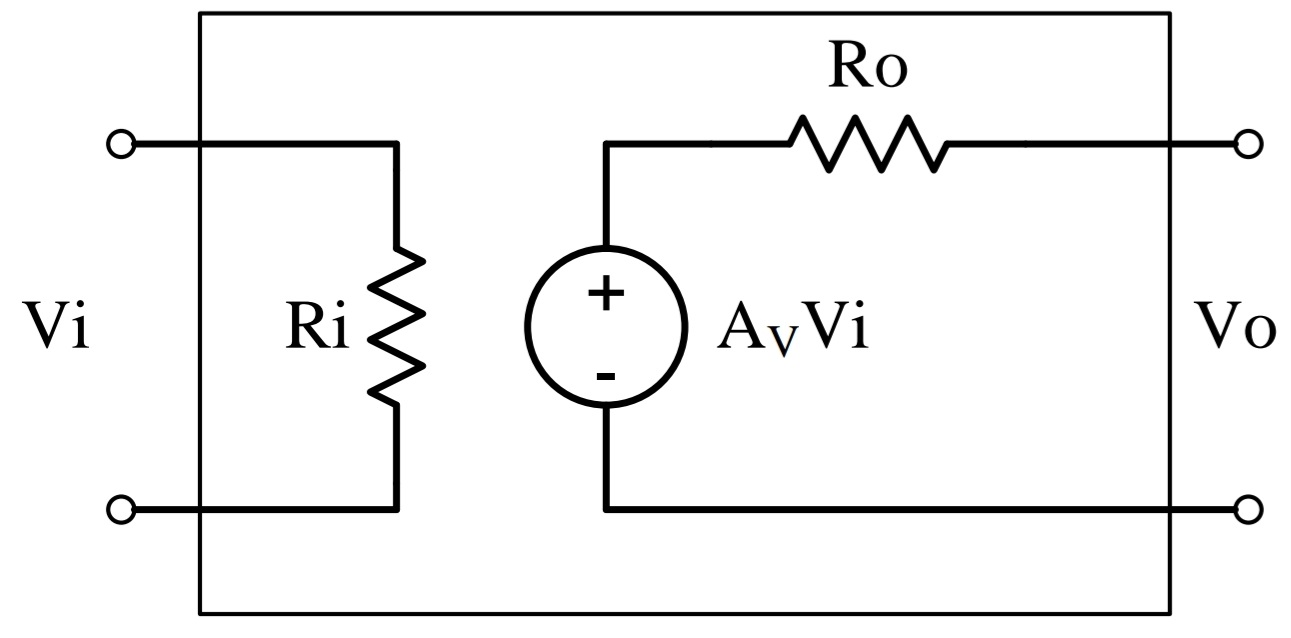
\includegraphics[height=5cm\textwidth]{zio.jpg}
        \caption{Modelo lineal de amplificador de tensión}
        \label{fig:zio}
    \end{figure}

    Para determinarlas resistencias de entrada y salida, $R_i$ y $R_o$ respectivamente, se colocan resistencias patrones $R_{PRi}$ y $R_{PRo}$ como se muestra en la Figura \ref{fig:rp} aproximadas según los valores estimados en los cálculos prévios de $R_i$ y $R_o$.

    \begin{figure}
        \centering
        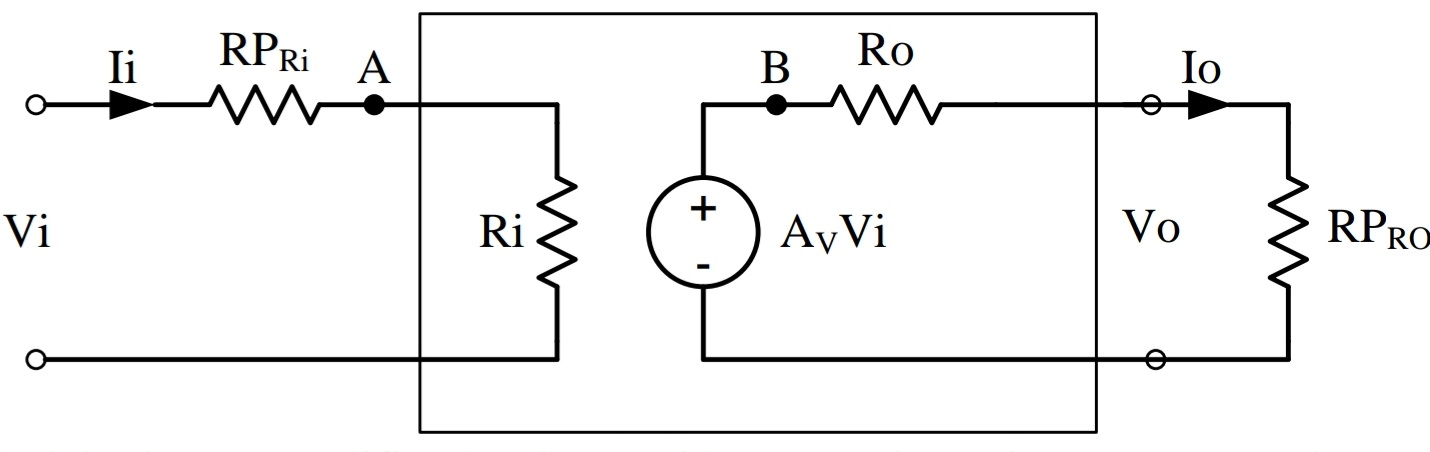
\includegraphics[height=5cm\textwidth]{RPdiagrama.jpg}
        \caption{Modelo lineal de amplificador de tensión con resistencias patrones de entrada y salida}
        \label{fig:rp}
    \end{figure}

    La corriente de entrada $I_i$ viene dada por

    $$I_i = {V_{R_{PRi}} \over R_{PRi}}$$

    También es igual a,

    $$I_i = {V_{R_{i}} \over R_{i}}$$

    Igualando ambas ecuaciones

    $${V_{R_{PRi}} \over R_{PRi}} = {V_{R_{i}} \over R_{i}}$$

    $$R_i = {V_{R_{i}} \over V_{R_{PRi}}}R_{PRi}$$

    Si $V_{R_{PRi}} = V_i - V_{R_{i}}$

    \begin{equation} \label{eqri}
        R_i = {V_{R_{i}} \over V_i - V_{R_{i}}}R_{PRi}
    \end{equation}

    Donde $V_{R_i}$ es la tensión en el punto A que se puede medir

    Para la resistencia de salida se procede de igual forma. La corriente $I_o$ viene dada por

    $$I_o = {V_{R_{PRo}} \over R_{PRo}}$$

    Por otra parte también

    $$I_o = {V_{R_o} \over R_o}$$

    Igualando ambas ecuaciones

    $${V_{R_{PRo}} \over R_{PRo}} = {V_{R_o} \over R_o}$$

    $$R_o = {V_{R_o} \over V_{R_{PRo}}}R_{PRo}$$

    $$R_o = {V_B - V_{R_{PRo}} \over V_{R_{PRo}}}R_{PRo}$$

    $V_{R_{PRo}}$ es la tension a la salida del amplificador

    $$R_o = {V_B - V_o \over V_o}R_{PRo}$$

    Al punto B de la figura \ref{fig:rp} no se tiene acceso y no se puede medir, pero esa tensión es la misma cuando el amplificador se encuentra sin carga ($V_{osc}$) y $V_o$ es la tensión con carga ($V_{occ}$), la ecuación para determinar la resistencia de salida del amplificador queda,

    \begin{equation} \label{eqro}
        R_o = {V_{osc} - V_{occ} \over V_{occ}}R_{PRo}
    \end{equation}



    \newpage

    Hojas de datos que contienen los valores experimentales recopilados en el laboratorio.

    \begin{figure}
        \centering
        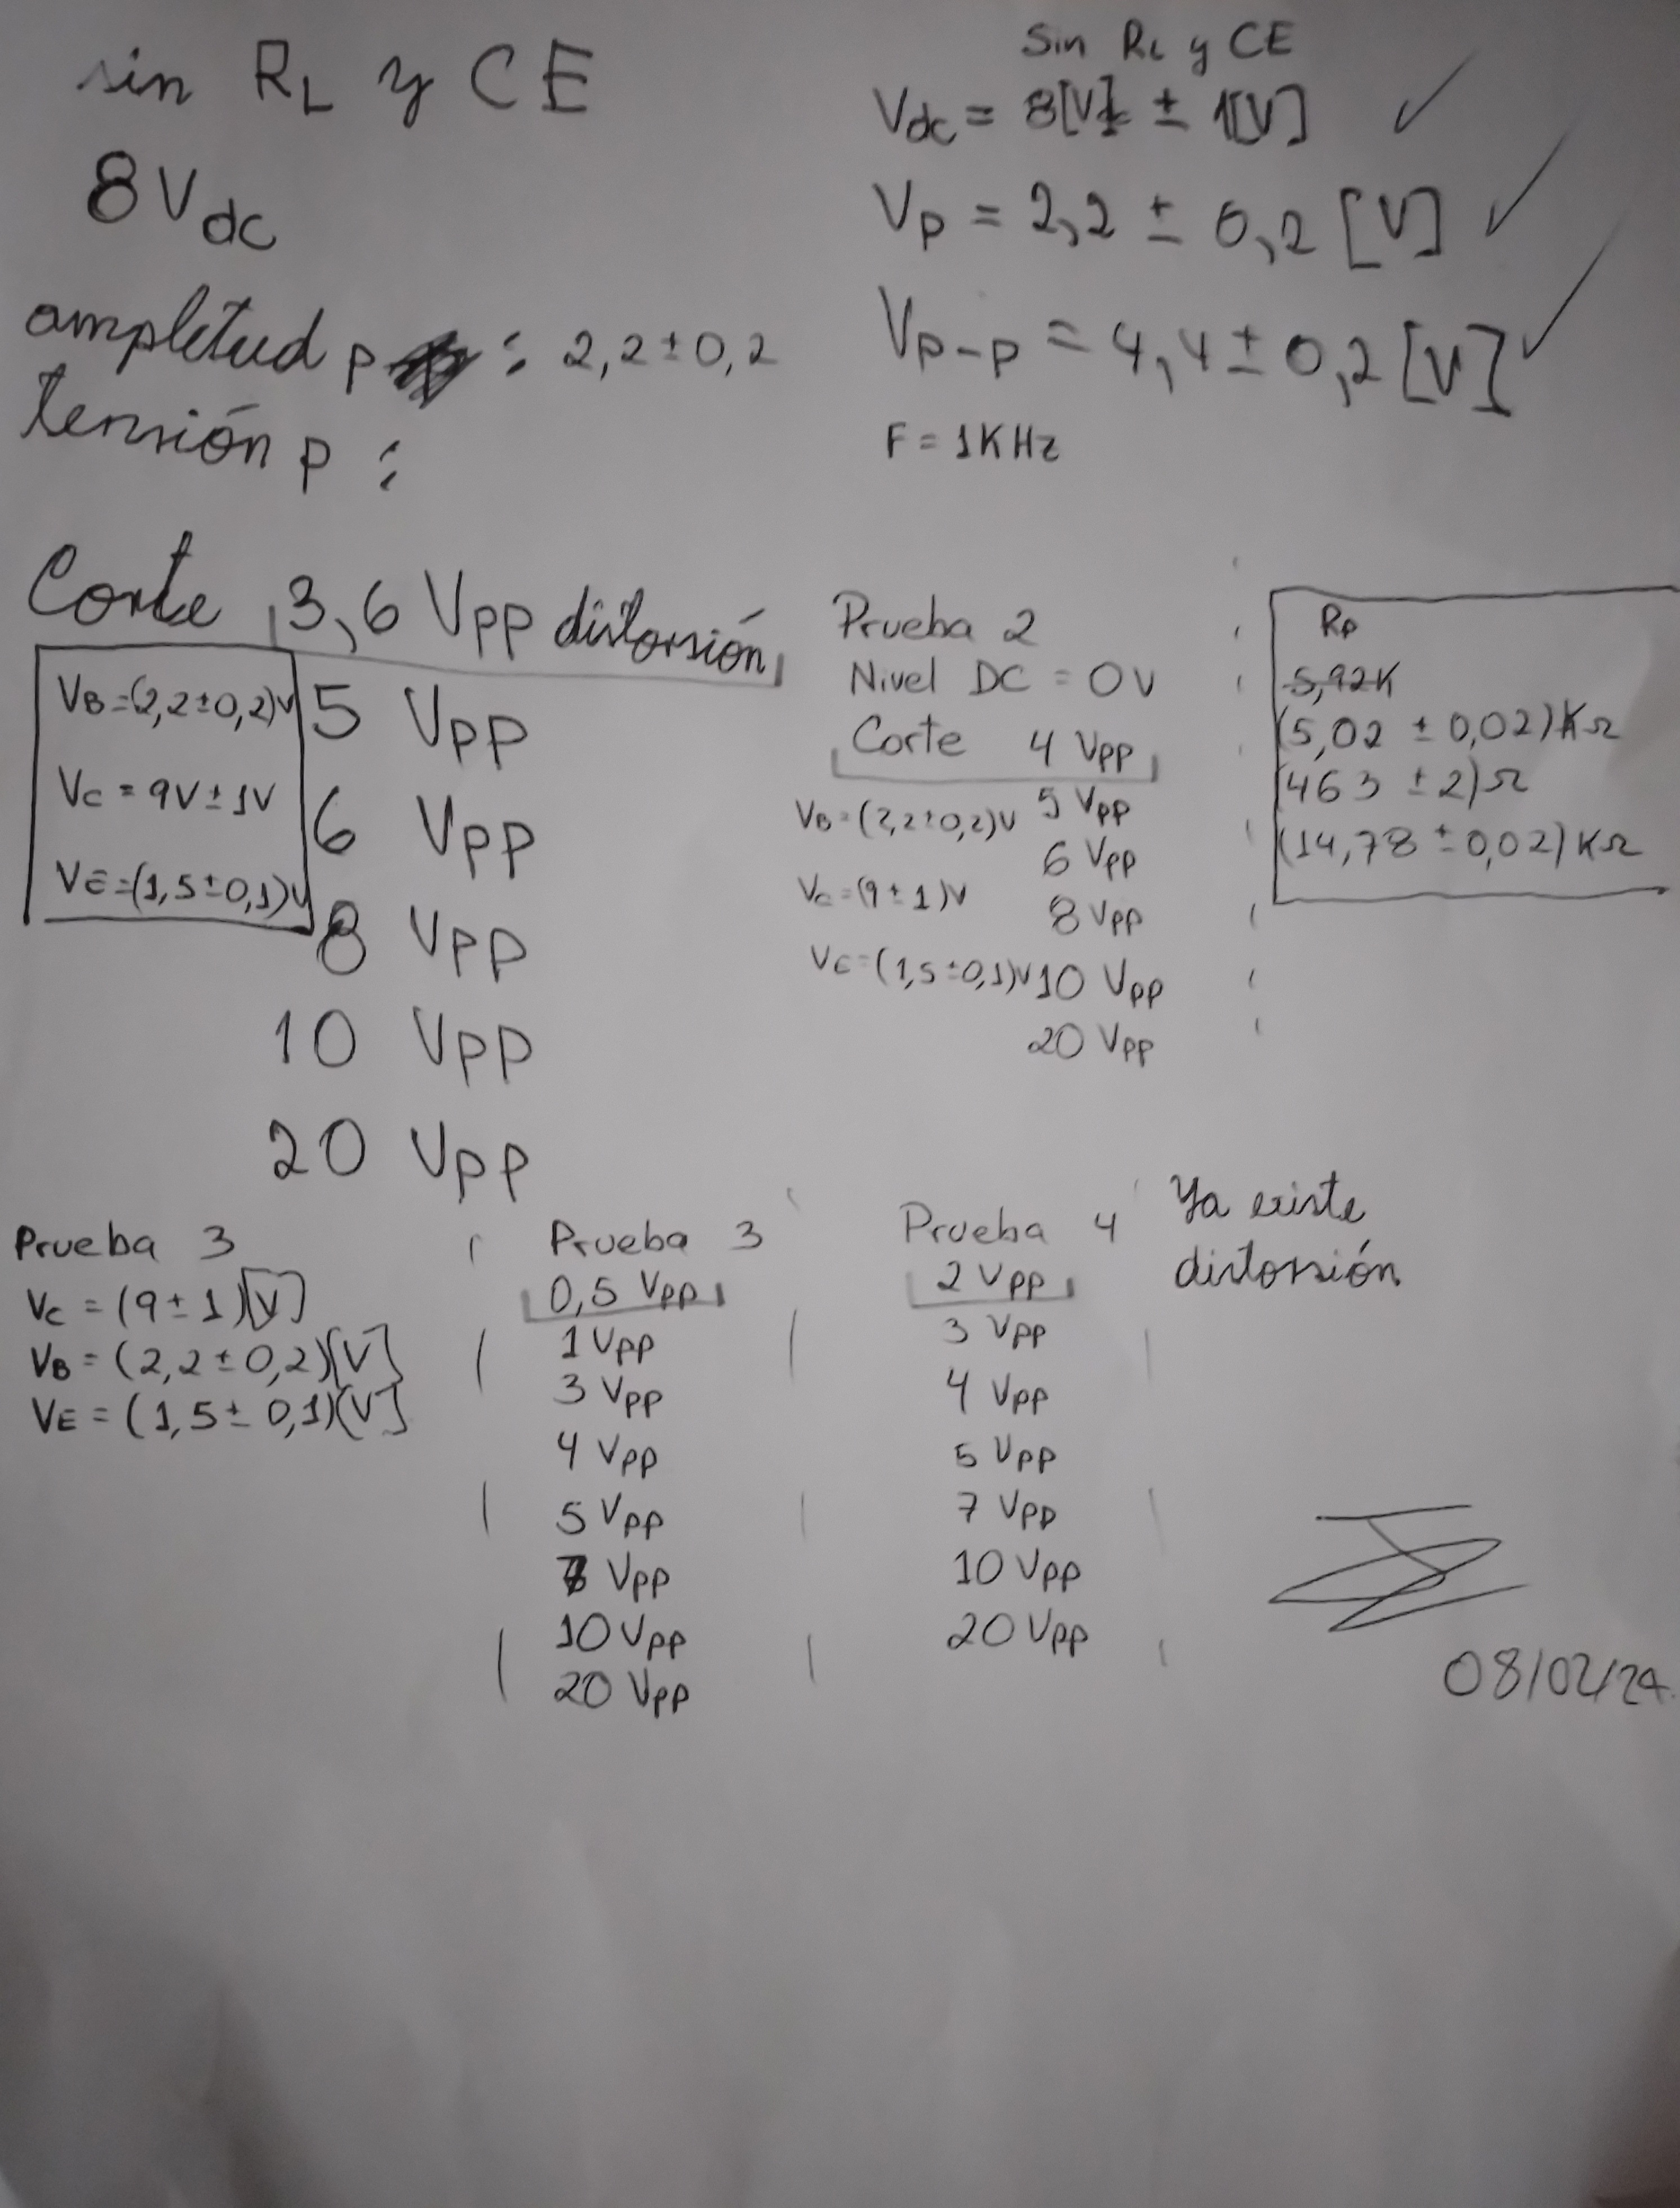
\includegraphics[height=10cm\textwidth]{hoda1.jpg}
        \caption{hoja de datos}
        \label{fig:hd1}
    \end{figure}


\end{document}